\documentclass[twoside,11pt]{article}

\usepackage{blindtext}

% Any additional packages needed should be included after jmlr2e.
% Note that jmlr2e.sty includes epsfig, amssymb, natbib and graphicx,
% and defines many common macros, such as 'proof' and 'example'.
%
% It also sets the bibliographystyle to plainnat; for more information on
% natbib citation styles, see the natbib documentation, a copy of which
% is archived at http://www.jmlr.org/format/natbib.pdf

% Available options for package jmlr2e are:
%
%   - abbrvbib : use abbrvnat for the bibliography style
%   - nohyperref : do not load the hyperref package
%   - preprint : remove JMLR specific information from the template,
%         useful for example for posting to preprint servers.
%
% Example of using the package with custom options:
%
% \usepackage[abbrvbib, preprint]{jmlr2e}

\PassOptionsToPackage{table}{xcolor}   % BEFORE \usepackage{jmlr2e}, which loads xcolor
\usepackage{jmlr2e}
\usepackage{pdlistings}
\usepackage{xcolor}
\usepackage{amsmath}
\usepackage{mathtools}
\usepackage{cleveref}
\usepackage{csquotes}
\usepackage{booktabs}
\usepackage{bm}
\hypersetup{hidelinks}
\renewcommand{\BlackBox}{\ensuremath{\square}}
\renewenvironment{proof}[1][Proof]{%
  \par\noindent\textbf{#1.}\enspace\ignorespaces
}{%
  \ifhmode\unskip\nobreak\hfill\quad\else\noindent\hfill\fi
  \BlackBox\par\addvspace{2mm}%
}
\makeatletter
\def\@begintheorem#1#2{%
  \trivlist
  \item[\hskip\labelsep{\normalfont\bfseries #1\ #2.}]\itshape
}
\def\@opargbegintheorem#1#2#3{%
  \trivlist
  \item[\hskip\labelsep{\normalfont\bfseries #1\ #2\ (#3).}]\itshape
}
\makeatother




\usepackage{tikz}
\usetikzlibrary{positioning,fit,arrows.meta,backgrounds,calc,matrix}





% Definitions of handy macros can go here

\usepackage{xcolor}
\definecolor{darkred}{rgb}{0.8, 0, 0}
\newcommand{\boldred}[1]{\textbf{\textcolor{darkred}{#1}}}
\newcommand{\boldblue}[1]{\textbf{\textcolor{blue}{#1}}}

\newcommand{\dataset}{{\cal D}}
\newcommand{\fracpartial}[2]{\frac{\partial #1}{\partial  #2}}

% Heading arguments are {volume}{year}{pages}{date submitted}{date published}{paper id}{author-full-names}

\usepackage{lastpage}
\jmlrheading{23}{2022}{1-\pageref{LastPage}}{1/21; Revised 5/22}{9/22}{21-0000}{Author One and Author Two}

% Short headings should be running head and authors last names

\ShortHeadings{Partial Transparency in OSGT}{Duclaux, Formenti and Cobben}
\firstpageno{1}

\begin{document}

\title{Partial Transparency in OSGT}

\author{\name Colomban Duclaux \email cduclaux@ethz.ch \\
       ETH Zürich\\
       Zürich, Switzerland
       \AND
       \name Author Two \email two@cs.berkeley.edu \\
       \addr Division of Computer Science\\
       University of California\\
       Berkeley, CA 94720-1776, USA}

\editor{My editor}

\maketitle

\begin{abstract}%   <- trailing '%' for backward compatibility of .sty file
\blindtext
\end{abstract}

\begin{keywords}
  keyword one, keyword two, keyword three
\end{keywords}

\tableofcontents

\section{Introduction}

\section{Related Work}
\label{section:RelatedWorks}

\boldred{[Papers that are important to cite and to-do:]}
\begin{itemize}
\item use google review product, potentially also worth using https://asta.allen.ai/ (not sure if it's still SOTA)
    \item Similarity-based cooperative equilibrium, Oesterheld
    \item A commitment folk theorem (cite near tennetholz)
    \item check GT literature
    \item why lean formalization? to make automatic proof search possible with AI agent; see verifiable rewards
    \item cite SCE 
    \item references url
    \item repository should have same set of authors
    \item AI usage statement
    \item gpt.zero + pangram
    \item references
    \item acknowledgments
    \item clean the repo
\end{itemize}


\newpage

\section{Theory}\label{sec:theory}

\boldred{TITLE}

\boldred{I wonder if we should do some high-level signposting of what we're going to do here. A nice birds eye view and motivation.}
\boldblue{Agreed, something like: \textit{Game theory, the mathematical theory of strategic decision-making \citep{game_theory}, models players interacting together in well-defined environments. However, classical game theory models each player as an independent actor with no particular knowledge of its opponents, and sometimes not even of the environment \citep{Harsanyi1,Harsanyi2,harsanyi3}. Open-source game theory unpacks this black-box assumption.
Before diving into the theoretical framework of open-source game theory, we introduce standard concepts from game theory that will be useful for the open-source version. For this, we follow the notations of \citet{duclaux2026proving}.}}


\boldred{check with gpt + claude}

\boldred{what to emph in the section}

\boldred{add a comment to emph that OSGT allows for cooperation in the PD}

A game $G$ in normal form is a tuple $G=(I, (A_i, u_i)_{i \in I})$, where $I$ is a finite set of players, $A_i$ is the finite set of actions available to player $i$, and $u_i:\prod_{j \in I} A_j \to \mathbb{R}$ is the utility (payoff) function of player $i$. For simplicity's sake, we restrict our attention to two players games with common action sets, i.e. $I=\{1,2\}$ and $A \coloneq A_1 = A_2$. As is customary, for player $i \in I$, let's denote by $-i$ the other player and by $\bm{a} \in A\times A$ an action profile. \boldblue{I would drop the mixed strategies as we don't use any in the experiments (We can mention it as a footnote for exhaustivity).} Finally, a mixed action for player $i \in I$ is a probability distribution over $A_i=A$, an element of the probability simplex $\Delta(A)$; we extend $u_i$ to $\Delta(A) \times \Delta(A)$  by expectation in the usual way. The (in)famous Prisoner's Dilemma will serve as the main example throughout.

\begin{example}[Prisoner's Dilemma]\label{example:PD}
The Prisoner's Dilemma is a two-player game $G_{\mathrm{PD}}$ with common action set $A = \{C, D\}$, cooperate (C) and defect (D), and payoffs
  \[
    \begin{array}{c|cc}
         & C     & D     \\ \hline
       C & (R,R) & (S,T) \\
       D & (T,S) & (P,P)
    \end{array}
    \qquad\qquad T > R > P > S,
  \]
  where rows are the actions of player~1, columns those of player~2, and each entry lists $(u_1, u_2)$.  Since $T > R$ and $P > S$, the action $D$ strictly dominates $C$ for each player. \boldblue{I would define Nash and maybe Pareto here, see master then.} Hence $(D,D)$ is the unique Nash equilibrium of $G_{\mathrm{PD}}$, even though $R > P$ means it is Pareto-dominated\footnote{For action profiles $\bm{a}$ and $\bm{a}' \in A \times A$, $\bm{a}$ is said to Pareto-dominate $\bm{a'}$ if for all $i$ in $I$, $u_i(\bm{a}) \ge u_i(\bm{a}')$, with strict inequality for some $j \in I$.  We say that $\bm{a}$ is Pareto-optimal if no other action profile Pareto-dominates it.} by $(C,C)$. \boldred{I'm not sure if footnotes inside a sentence are usual, maybe @riccardo you could let me know? Usually I see them afterwards}
\end{example}

\boldblue{Add OSGT motivation here (see master thesis)}
Suppose that, instead of choosing an action directly, each player submits a computer program that takes the other players' programs as input and outputs an action. Executing these programs produces an action profile. In particular, a player's program may then condition its action on a formal inspection of the opponents' programs, and conditional commitments of the form ``cooperate if and only if I can verify that you will cooperate'' in Example~\ref{example:PD} become well-defined objects of strategic choice. \boldred{I would potentially simplify the previous sentence } This setting was first introduced by \cite{tennenholtz2004program}, and later termed Open Source Game Theory (OSGT) by \cite{Critch}.

\subsection{Open Source Game Theory}\label{sec:osgt}

To make precise the meta-game in which players commit to a program instead of directly playing an action, we build on the formalization and notation of \cite{duclaux2026proving}. For each player $i \in I$, denote by $\Sigma_i$ the finite set of admissible programs. Again, we assume common program sets, that is, $\Sigma \coloneq \Sigma_1 = \Sigma_2$, and we denote by $\bm{\pi}= (\pi_1, \pi_2) \in \Sigma \times \Sigma$ a program profile. Each program receives its opponent's program as input.\footnote{Throughout, we fix a computable injective encoding of finite program descriptions into $\mathbb{N}$ and, when no confusion arises, identify each program with its code.} We deliberately leave admissibility under-specified at this point, with the only requirement being that every admissible program, run on any admissible program (including itself), halts and returns an action. \boldred{A concrete choice of Sigma is later given ... [cite lean]}

\boldblue{Not sure how relevant it is to isolate-define \enquote{Mutually halting program set} if we don't specify it. I would instead define the run function and speak about mutually halting program set in that definition. Then add outcome as a new definition. Or you just define everything in prose.} 
\begin{definition}[Mutually halting program set]\label{def:mutually-halting}
  A common program set $\Sigma$ is mutually halting if, for all $\pi, \pi' \in \Sigma$, the execution of $\pi$ on input $\pi'$ terminates and outputs an action in $A$. In this case, the execution function $\operatorname{run} \colon \Sigma \times \Sigma \to A$ maps $(\pi, \pi')$ to that output, which we write suggestively as
  $\operatorname{run}(\pi \mathrel{\|} \pi')$. 
\end{definition}

Moreover, we assume that every constant program is admissible, that is, for each action $a \in A$, the program that ignores its input and always plays $a$ belongs to $\Sigma$. \boldred{Maybe I'm mistaken, is this an assumption? I guess maybe a diferent bot could have a constant bot as input and idk die?} With an abuse of notation, we denote this program by $a$, so that $\operatorname{run}(a \|\pi) = a$ for all $\pi \in \Sigma$, and we define a natural embedding $A \subseteq\Sigma$. This assumption and the mutually halting condition of Definition~\ref{def:mutually-halting} will be assumed throughout without further mention. 

The execution function $\operatorname{run}$ induces the outcome map of the game, which to a profile of programs assigns its played action profile
\begin{equation*}
    \operatorname{outcome}:\Sigma \times \Sigma \to A \times A, \quad \mathrm{outcome}(\bm{\pi}) \coloneq \biggl(\mathrm{run}(\pi_1 \| \pi_2), \mathrm{run}(\pi_2 \|\pi_1)\biggr),
\end{equation*}
which assigns to each program profile $\bm{\pi} = (\pi_1, \pi_2)$ the action profile it produces. Each player utility is then naturally extended to program profiles, 
\begin{equation*}
    U_i: \Sigma \times \Sigma \to \mathbb{R},
\qquad
U_i(\bm{\pi}) \coloneq u_i\bigl(\operatorname{outcome}(\bm{\pi})\bigr).
\end{equation*}
Since $A \subseteq \Sigma$ and constant programs play their constant action against any opponent, the meta-utility $U_i$ indeed restricts to $u_i$ on $A \times A$. The tuple $G^{\mathrm{prog}} := \bigl(I, (\Sigma_i, U_i)_{i \in I}\bigr)$ constitutes a normal form game, which we call the program meta-game associated with $G$. \boldblue{\enquote{As for classical game theory, we have a open-source version of rational play...}}We are ready to give the definition of equilibrium introduced by \cite{tennenholtz2004program} for program meta-games.

\begin{definition}[Program Equilibrium]\label{def:PE}
A profile $\bm{\pi}^{*} \in \Sigma \times \Sigma$ is a Program Equilibrium (PE) of $G$ if it is a (pure) Nash equilibrium of $G^{\mathrm{prog}}$, i.e., for every $i \in I$ and every $\pi_i' \in \Sigma$,
\[
U_i(\pi_i^{*}, \pi_{-i}^*) \;\ge\; U_i(\pi_i',\, \pi^{*}_{-i}).
\]
\boldblue{Same, I would remove this.} More generally, a profile $\bm{\alpha}^* \in  \Delta(\Sigma) \times \Delta(\Sigma)$ is a mixed Program equilibrium if it is a mixed Nash equilibrium of $G^{\mathrm{prog}}$, where we have extended $U_i$ by expectation.
\end{definition}

We first observe that if the underlying game $G$ admits a pure Nash equilibrium, then so does the meta-game $G^{\mathrm{prog}}$. In fact, it suffices to replace each equilibrium action by the corresponding constant program. All proofs for this Section are deferred to Appendix~\ref{sec:app:proof}.

\begin{theorem}[Pure Nash equilibria are program equilibria]\label{th:NE-is-PE}
Let $\bm{a}^* \in A \times A$ be a pure Nash equilibrium of $G$. Then the profile of constant programs $\bm{a}^* \in \Sigma \times \Sigma$ is a pure  program equilibrium of $G$.
\end{theorem}

\boldblue{Same, I would remove this.} More generally, existence does not depend on $G$ having a pure equilibrium. Since $\Sigma$ is finite and nonempty (it contains $A$), the meta-game $G^{\mathrm{prog}}$ is a finite normal-form game, so by Nash's existence theorem \citep{nash1950equilibrium, nash1951} it admits a mixed Nash equilibrium $\bm{\alpha}^* \in \Delta(\Sigma) \times \Delta(\Sigma)$. By definition, $\bm{\alpha}^*$ is a mixed program equilibrium of $G$.

\boldblue{I would move this example below so that we directly speak of Dupoc to justify why it plays such a central role in OSGT. We can mention CliqueBot but it is not so important.}
\begin{example}[Prisoner's Dilemma, cont’d]
  By Theorem~\ref{th:NE-is-PE}, mutual defection $(D,D)$ remains a program equilibrium of $G_{\mathrm{PD}}$. \boldred{Next sentence I think has some grammar issues} Unlike in the Prisoner's Dilemma, however, it is no unique as Program equilibria can also sustain cooperation. The simplest example is Tennenholtz's \texttt{CliqueBot} \citep{tennenholtz2004program}, which cooperates if its input is syntactically identical to its own code and defects otherwise. If \texttt{CliqueBot} is admissible, then the profile (\texttt{CliqueBot}, \texttt{CliqueBot}) yields $(C,C)$. Any unilateral deviation $\pi'$ obtains defection, so it earns $\max\{S,P\} = P < R$. The proof-based bots introduced by \cite{Critch} show that cooperation can also be achieved by programs robust to syntactic differences, such as \texttt{DupocBot}, which we recall below.
\end{example}

In this paper we focus our attention on proof-based OSGT~\citep{Modal_agents_barasz,Critch}, where programs will have access to a formal proof system $S$ (e.g. Peano Arithmetic) to be later specified \boldred{[reference section]} in which to state hypotheses about their opponents and search for proofs of them\footnote{Another paradigm of OSGT is simulation-based OSGT, where programs simulate their opponent instead of formulating mathematical proofs \citep{oesterheld2019robust, DBLP:conf/ijcai/KovarikOC23, DBLP:conf/aaai/CooperOC25}. Simulation and provability are two sides of the same coin, as a successful simulation is a concrete computational proof of a simulated program's behavior. Our library of programs thus allows for both kinds of bots. However, naive mutual simulation can lead to infinite recursion, and thus we focus this paper on proof-based programs.}. In particular, we use a proof search function that searches for a proof of a statement $\varphi$ in $S$ depending on a program $\pi' \in \Sigma$, of length at most $k \in \mathbb{N}$.
\begin{lstlisting}[style=pdcode, mathescape=true]
def proof_search($k, \pi', \varphi$):
    # Returns True iff $S$ has a proof of $\varphi$ about $\pi'$ of length at most $k$.
\end{lstlisting}
\boldblue{I would put this in the S theory section, because there we show all the properties of our tools.} By construction, \texttt{proof\_search}$(k, \pi', \varphi)$ returns \texttt{True} exactly when $S$ has a proof of $\varphi$ of length at most $k$. We require throughout that $S$ be sound, i.e., whatever $S$ proves is true. This implies that if the search succeeds, then $\varphi$ holds, and, in particular, $\pi'$ actually does what $\varphi$ says it does.

\begin{example}[Prisoner's Dilemma, cont’d]\label{ex:prisonerdilemma-3}
 Consider $G_{\mathrm{PD}}^{\mathrm{prog}}$, the program meta-game induced by the Prisoner's Dilemma. The canonical example of a provability-based program is \emph{\texttt{DupocBot}}$(k)$, for $k \in \mathbb{N}$, \enquote{Defect Unless Proof of Cooperation}, which on an opponent $\pi \in \Sigma$,
\begingroup
\upshape
\begin{lstlisting}[style=pdcode, mathescape=true]
def DupocBot$(k)(\pi)$:
   if proof_search($k, \pi, \mathrm{run}(\pi \| \mathrm{DupocBot}(k) ) = C$):
        return C
   else:
        return D
\end{lstlisting}
\endgroup
The interest of this program lies in the fact that it cooperates with cooperative opponents, but never gets exploited\footnote{This is a simple consequence of soundness of the formal proof system $S$ (see \cref{apx-subsubsection:Theory-AddResultsCritch-Unexploitability}).}, i.e. never cooperates when the other defects. The difficulty in proof-based OSGT lies in the logical and strategic interactions between programs that prove propositions about other programs. As an example, consider the following:
\begingroup
\upshape
\[
\mathrm{outcome}(\mathrm{\texttt{DupocBot}}(k), \mathrm{\texttt{DupocBot}}(k))
\]
\endgroup
It is not immediately clear what the result should be. Both programs are identical, and try to prove that their opponent cooperates. As \citet{Critch} put it, we face am apparent circular dependency: \enquote{the only way \emph{\texttt{DupocBot}}$(k)$ returns $C$ is if it first finds a proof in fewer than $k$ characters that \emph{\texttt{DupocBot}}$(k)$ returns $C$!} Intuitively, one might argue that for cooperation to occur, \emph{\texttt{DupocBot}}$(k)$ would have to prove that \emph{\texttt{DupocBot}}$(k)$ proves that \emph{\texttt{DupocBot}}$(k)$ proves that... and such a proof could not exist in finite length $k$. So one might expect that $\mathrm{outcome}(\emph{\texttt{DupocBot}}$(k)$, \emph{\texttt{DupocBot}}$(k)$) = (D, D)$. Quite surprisingly, this is not the case; \cite{Critch} show that for large $k$ the outcome is in fact mutual cooperation $(C, C)$, using an argument via the Parametric Bounded L\"ob Theorem (PBLT) \boldred{is it 2019 or 2022?}~\citep[Theorem~4.2]{Critch_pblt}. For such $k$, assuming \emph{\texttt{DupocBot}}$(k) \in \Sigma$, the profile (\emph{\texttt{DupocBot}}$(k)$, \emph{\texttt{DupocBot}}$(k)$) is a program equilibrium; in fact, each player receives $R$, and soundness of $S$ rules out unilateral deviations. Thus mutual cooperation is sustained as an equilibrium outcome of the Prisoner's Dilemma. \boldblue{Somewhere in this example mention section on formal S where we detail all this.}
\end{example}

It is important to note how transparency of the opponent’s source code can support program equilibria whose played actions, such as mutual cooperation in the Prisoner’s Dilemma (see Example~\ref{ex:prisonerdilemma-3}), cannot be supported in equilibrium in the underlying game. By conditioning cooperation on verifiable properties of the opponent’s program, players can make cooperation robust to unilateral deviations. 

\subsection{Partial Transparency}

The classical framework of open-source game theory described in Section~\ref{sec:osgt} assumes full transparency, in that each program receives the opponent's exact program as input. This is a strong descriptive assumption. In most settings of practical interest, players have only partial access to one another; for instance, a deployed model may be queried as a black box without exposing its weights, or agents may know little more than that they belong to the same base model family or company. Partial transparency of this kind motivates the diff meta games of \cite{DBLP:conf/nips/OesterheldTGCF23}. In these games, each program observes a single scalar measure of similarity between itself and the opponent's program and maps this signal to a mixed action. \boldred{possibly this goes in the intro}

More importantly, the literature treats transparency as an exogenous feature of the environment. Instead, we adopt here the perspective a designer who controls the players' informational environment, that is, controls what each program may observe about its opponent, in the spirit of information design \boldred{cite information design bergmann}. Our motivating application is AI safety. Training protocols (e.g. debate \boldred{cite}) and deployment protocols (e.g. oversight \boldred{cite}) rely on agents challenging or evaluating one another. If those agents collude and pursue objectives that conflict with the designer's preferences, the effectiveness of the above methods might be undermined \boldred{I think this is great. I am inclned to put this in the intro as well as our motivating example?}\boldblue{Agreed but this does not necessarily underline the \endquote{partial} part of transparency, more just transparency in general, i.e OSGT.}\footnote{By collusion we mean that the agents coordinate on an outcome that benefits them with respect to their own, possibly misaligned, preferences but that is contrary to the purpose of the protocol.  When each agent is individually tempted to report, the interaction is a Prisoner's Dilemma and collusion is mutual cooperation.}. This motivates studying partial transparency as a design variable in proof-based OSGT.

As in Section~\ref{sec:osgt}, we fix a finite base game $G$ and a finite set $\Sigma$ of admissible programs, shared by both players and common knowledge between them. Now, however, a program no longer receives the opponent's program as input. Instead, it receives a probability distribution $\mu \in \Delta(\Sigma)$, interpreted as the program's belief about which program the opponent has actually submitted. We therefore extend Definition~\ref{def:mutually-halting} to allow beliefs as inputs.

\boldblue{Again, I would not necessarily emphasize mutual halting, but more the belief, and the run function.}
\begin{definition}[Mutually halting program set; belief inputs]\label{def:mutually-halting-2}
  A common program set $\Sigma$ is mutually halting if, for all $\pi \in \Sigma$ and all beliefs $\mu \in \Delta(\Sigma)$, the execution of $\pi$ on input $\mu$ terminates and outputs an action in $A$. In this case, the execution function $\operatorname{run} \colon \Sigma \times \Delta(\Sigma) \to A$ maps $(\pi, \mu)$ to that output, which we write suggestively as
  $\operatorname{run}(\pi \mathrel{\|} \mu)$.
\end{definition}

As in Section~\ref{sec:osgt}, we assume that every constant program is admissible, that is, for each action $a \in A$, the program that ignores its input belief and always outputs $a$ belongs to $\Sigma$. We again denote this program by $a$, so that $\operatorname{run}(a \| \mu) = a$ for every $\mu \in \Delta(\Sigma)$, and we retain the embedding $A \subseteq \Sigma$.

\boldblue{$\tau$ already used for transposition so need to discuss the notation standards.}
The information structure of the game is described by a pair of transparency maps $\tau = (\tau_1, \tau_2)$, where $\tau_i \colon \Sigma \to \Delta(\Sigma)$ for each $i \in I$. Here $\tau_i(\pi)$ is the belief that player $i$'s program receives as input when the opponent $-i$ submits $\pi$. Intuitively, $\tau_i$ describes what player $i$'s program can learn about its opponent, for instance through black-box queries or knowledge of a shared model family, and it is the object the designer controls. At one extreme, $\tau_i(\pi) = \delta_\pi$ recovers the full transparency of Section~\ref{sec:osgt}; at the other, a constant $\tau_i$ reveals nothing, and player $i$ effectively chooses an action of the base game $G$; for more details, see Section~\ref{sec:more-less-transparency}.

Naturally extending the definitions of Section~\ref{sec:osgt}, we define the outcome map induced by the execution function $\operatorname{run}$ and the transparency maps $\tau$,
\begin{equation*}
    \operatorname{outcome}^\tau:\Sigma \times \Sigma \to A \times A, \quad \mathrm{outcome}^\tau(\bm{\pi}) \coloneq \biggl(\mathrm{run}(\pi_1 \| \tau_1(\pi_2)), \mathrm{run}(\pi_2 \| \tau_2(\pi_1))\biggr),
\end{equation*}
which assigns to each program profile $\bm{\pi} = (\pi_1, \pi_2)$ the action profile it produces. The only change from Section~\ref{sec:osgt} is that each program now runs on the belief it receives from the opponent's code. Each player's utility is then extended to program profiles by 
\begin{equation*}
    U_i^\tau: \Sigma \times \Sigma \to \mathbb{R},
\qquad
U_i^\tau(\bm{\pi}) \coloneq u_i\bigl(\operatorname{outcome}^\tau(\bm{\pi})\bigr).
\end{equation*}
The tuple $G^\tau \coloneqq \bigl(I, (\Sigma_i, U_i^\tau)_{i \in I}\bigr)$ is a normal-form game, which we call the \emph{$\tau$-program meta-game} associated with $G$; the superscript makes its dependence on the transparency maps $\tau$ explicit. Following Definition~\ref{def:PE}, a profile $\bm{\pi} \in \Sigma \times \Sigma$ is a $\tau$-Program Equilibrium (or simply a Program Equilibrium, when $\tau$ is clear from context) if it is a pure Nash equilibrium of $G^\tau$; mixed $\tau$-Program Equilibria are defined analogously.

\begin{definition}[$\bm{\tau}$-Program Equilibrium]\label{def:tau-PE}
A profile $\bm{\pi}^{*} \in \Sigma \times \Sigma$ is a $\tau$-Program Equilibrium (PE) of $G$ if it is a (pure) Nash equilibrium of $G^\tau$, i.e., for every $i \in I$ and every $\pi_i' \in \Sigma$,
\[
U_i^\tau(\pi_i^{*}, \pi_{-i}^*) \;\ge\; U_i^\tau(\pi_i',\, \pi^{*}_{-i}).
\]
\end{definition}

\begin{theorem}[Pure Nash equilibria are $\bm{\tau}$-program equilibria]\label{th:NE-is-tau-PE}
Let $\tau$ be any pair of transparency maps and let $\bm{a}^* \in A \times A$. Then the profile of constant programs $\bm{a}^* \in \Sigma \times \Sigma$ is a pure $\tau$-Program Equilibrium if and only if $\bm{a}^*$ is a pure Nash equilibrium of $G$. In particular, every pure Nash equilibrium of $G$ is a $\tau$-Program Equilibrium for every choice of $\tau$.
\end{theorem}

\boldblue{Remove if we remove mixed strategies in GT.}
More generally, the existence of $\tau$-Program Equilibria does not depend on $G$ having a pure equilibrium, as one can apply Nash's existence theorem \citep{nash1950equilibrium, nash1951} to $G^\tau$ to prove existence of a mixed $\tau$-Program Equilibrium of $G$.

\subsection{When Does Transparency Matter?}\label{sec:more-less-transparency}

Rational behaviour in the meta game $G^\tau$ can differ from rational behaviour in the base game $G$ only insofar as $\tau$ reveals something about how programs behave. To make this precise, consider a player who can mimic, that is, for any of her programs $\pi$, any belief $\mu$ that her programs may receive, and any target action $x$, she can find a program $\rho$ that her opponent cannot distinguish from $\pi$ and that plays $x$ on input $\mu$.

\begin{definition}[Mimic]\label{def:mimic}
    Player $i \in I$ can mimic if for every $\pi \in \Sigma$, every $\mu \in \tau_i(\Sigma)$, and every $x \in A$ there exists a $\rho \in \Sigma$ such that
    \begin{enumerate}
        \item $\rho$ is indistinguishable from $\pi$ to player $-i$, that is, $\tau_{-i}(\rho) = \tau_{-i}(\pi)$;
        \item $\rho$ plays $x$ on input $\mu$, that is, $\mathrm{run}(\rho \| \mu)=x$.
    \end{enumerate}
\end{definition}

A program of player $-i$ can condition its action only on the belief it receives, $\tau_{-i}(\pi_i)$, and can therefore reward or punish player the opponent $i$ only through what is revealed by this belief. If $i$ can mimic, any arbitrary change in $i$'s behaviour can be made without changing what $-i$ observes. Hence no program of $-i$ can make its response depend on what $i$ actually does\footnote{Black-box testing provides a concrete example. If player $-i$ observes only how player $i$'s program behaves on a set of test inputs, then $i$ can mimic at every input outside this set. Testing can therefore deter opportunistic behavior only if the inputs a program faces in the actual interaction cannot be distinguished from test inputs. This the concern we face with evaluation awareness in AI systems.}; as Theorem~\ref{th:mimic} shows, this implies that the program meta-game reduces to the base game. This idea is the analogue of the informativeness principle in moral hazard \citep{holmstrom1979moral}; an additional signal can improve the optimal contract if and only if it provides information about the agent's action beyond what is already observed in the outcome.

\begin{theorem}\label{th:mimic}
    Assume player $i \in I$ can mimic. If $\bm{\pi} \in \Sigma \times \Sigma$ is a pure $\tau$-program equilibrium with outcome $\bm{a}$ then $a_i \in \mathrm{BR}_i(a_{-i})$, where $\mathrm{BR_i}$ is the best-response correspondence defined by
    \begin{equation*}
        \mathrm{BR}_i(a_{-i}) \coloneq \mathrm{argmax}_{a' \in A}u_i(a', a_{-i}).
    \end{equation*}
    Moreover, if both players can mimic, then the outcomes of pure $\tau$-program equilibria are exactly the pure Nash equilibria of $G$.
\end{theorem}

The two extreme transparency structures illustrate the result. If $\tau_{-i}$ is constant, so that player $-i$ observes nothing about $i$'s program, then player $i$ can trivially mimic (using the $x$-constant program). When $\tau$ is constant, Theorem~\ref{th:mimic} shows that the outcomes of pure $\tau$-PE are exactly the pure Nash equilibria of $G$; in this case, each player effectively chooses an action of the base game. On the other hand, full transparency, $\tau_i(\pi) = \delta_\pi$, recovers the open-source setting of Section~\ref{sec:osgt}. There mimicry fails\footnote{Definition~\ref{def:mimic} imposes a simple counting constraint. Fix any $\mu \in \tau_i(\Sigma)$ and any $\pi \in \Sigma$. Applying the definition to $(\pi, \mu, x)$ for each $x \in A$ yields programs $\rho_x$ with $\tau_{-i}(\rho_x) = \tau_{-i}(\pi)$ and $\mathrm{run}(\rho_x \,\|\, \mu) = x$, which are distinct for distinct $x$. Hence every set of programs that player $-i$ cannot distinguish from one another contains at least $|A|$ elements. Since these sets partition $\Sigma$ and there are $|\tau_{-i}(\Sigma)|$ of them,
\begin{equation*}
    |\tau_{-i}(\Sigma)| \cdot |A| \le |\Sigma|.
\end{equation*}
In particular, if $\tau_{-i}$ is injective, as under full transparency $\tau_{-i}(\pi) = \delta_\pi$, player $i$ cannot mimic as soon as $|A| \ge 2$. This is consistent with Section~\ref{sec:osgt}, where program equilibria can induce outcomes that are not Nash equilibria of $G$ (Example~\ref{ex:prisonerdilemma-3}).}, and program equilibria can sustain outcomes that are not Nash equilibria of $G$, such as mutual cooperation in the Prisoner's Dilemma (Example~\ref{ex:prisonerdilemma-3}). 

By varying the transparency map $\tau$, we thus obtain a family of games ranging from the base game $G$ to the fully transparent meta-game $G^{\mathrm{prog}}$ of \cite{tennenholtz2004program}; moreover, Theorem~\ref{th:NE-is-tau-PE} shows the inclusion $\mathrm{NE}\subseteq \mathrm{PE}$. Whether the corresponding sets of program equilibrium (or of outcomes) vary monotonically in $\tau$ under a suitable order on transparency maps is an interesting question we do not approach here. For this exercise, the results of \cite{battigalli2016analysis,formenti2026selfconfirming} may be useful.

















\subsection{An Example in the Prisoner's Dilemma}

We now return to our running example, the Prisoner's Dilemma (Examples~\ref{example:PD} and~\ref{ex:prisonerdilemma-3}), and illustrate partial transparency through concrete transparency maps and explicit programs. We assume throughout a common transparency map $\tau_1 = \tau_2$ for the two players; write $\tau$ for it.

Given a program \texttt{Bot} of the open source Prisoner's Dilemma $G_{\mathrm{PD}}^{\mathrm{prog}}$, we can extend it to a program \texttt{TauBot} of the meta-game $G_{\mathrm{PD}}^{\tau}$, which takes a belief $\mu \in \Delta(\Sigma)$ as input. In particular, \texttt{TauBot} runs the decision procedure of \texttt{Bot} against each program in the support of $\mu$ and aggregates the resulting actions. The simplest aggregator is a threshold rule, where for $\alpha \in [0,1]$, cooperate if and only if the $\mu$-mass of the programs against which \texttt{Bot} would cooperate is at least $\alpha$. We give below the example of \texttt{TauDupoc}$(k, \alpha)$.

\begin{lstlisting}[style=pdcode, mathescape=true]
def TauDupocBot$(k, \alpha)(\mu)$:
   mass = 0
   for $\pi'$ in $\operatorname{supp}(\mu)$:
        if proof_search($k, \pi', \mathrm{run}(\pi' \| \delta_{\mathrm{TauDupocBot}(k, \alpha)}) = C$):
             mass = mass + $\mu(\pi')$
   if mass $\geq \alpha$:
        return C
   else:
        return D
\end{lstlisting}

Unlike \texttt{DupocBot}$(k)$, \texttt{TauDupocBot}$(k, \alpha)$ is no longer unexploitable. Soundness of $S$ still guarantees that every program counted in \texttt{mass} cooperates on the point-mass input $\delta_{\texttt{TauDupocBot}(k,\alpha)}$, but for poorly behaved transparency map $\tau$, the actual opponent need not be one of these programs nor receive it as input.

\boldblue{Why not, but need to expand on this if we keep this, because right now it is not very clear.}
The threshold rule given above is linear in $\mu$ and therefore admits an expected utility representation\footnote{This holds on the state space $\Sigma$ and the larger consequence space $\{C,D\} \times \{0,1\}$, and let playing $a$ against $\pi$ give the consequence $(a, f(\pi))$, where $f(\pi) = 1$ if \texttt{TauBot} cooperates on the point-mass input $\delta_\pi$ and $f(\pi) = 0$ otherwise.}; non-linear aggregators, such as the maximum or minimum or a variational functional, capture ambiguity-sensitive behaviour \citep{gilboa2016ambiguity}. We do not explore their properties here.

\boldblue{Already in the appendix and the experiments.}
We conclude the section with examples of transparency maps to which we return in \boldred{Section}. Fix a finite program library $\Sigma = \{\pi_1, \ldots, \pi_n\}$ of admissible programs and assume that $\mathrm{outcome}(\pi_j,\pi_\ell)$ is known for every ordered pair. We consider here softmax-based transparency maps induced by a pseudo-distance on $\Sigma$.

\begin{definition}\label{def:tau-softmax-Family}
Let $d : \Sigma \times \Sigma \to \mathbb{R}_{\ge 0}$ be a pseudo-distance. For a temperature $T > 0$, the transparency map $\tau^{T}_{d}\colon \Sigma \to \Delta(\Sigma)$ is the softmax of $-d/T$:
\[
  \tau^{T}_{d}(\pi_j)(\pi_\ell)
  := \frac{\exp\bigl(-d(\pi_j,\pi_\ell)/T\bigr)}
          {\sum_{m=1}^{n} \exp\bigl(-d(\pi_j,\pi_m)/T\bigr)},
  \qquad \pi_j, \pi_\ell \in \Sigma.
\]
As is usual, we extend to $T = \infty$ by $\tau^{\infty}_{d}(\pi_j) = \mathrm{unif}_{\Sigma}$ and to $T= 0$ by $\tau^{0}_{d}(\pi_j) = \delta_{\pi_j}$, the full transparency of Section~\ref{sec:osgt}.
\end{definition}

A first example is the behavioral pseudo-distance, given by the Hamming distance between outcome rows. For $\pi \in \Sigma$, let $\mathrm{row}(\pi) := \bigl(\mathrm{outcome}(\pi, \pi_m)_1\bigr)_{m=1}^{n} \in A^n$ be the list of actions played by $\pi$ against the programs of the library, and define
\[
  d_{\mathrm{bvr}}(\pi_j, \pi_\ell) := \bigl|\{ m : \mathrm{row}(\pi_j)_m \neq \mathrm{row}(\pi_\ell)_m \}\bigr| \in \{0, \ldots, n\}.
\]
This is only a pseudo-distance, since distinct programs may have identical rows. Further examples arise from syntactic pseudo-distances, such as the tree edit distance between the abstract syntax trees of the programs' source code, computed with the Zhang-Shasha algorithm \boldred{cite}.

\boldred{see appendix}




\newpage

\section{Experiments}

\boldred{TITLE}

\boldred{intro}

\subsection{Full Transparency}

\boldred{TITLE}

We start by studying the base case, i.e. the full transparency of open source game theory. We fix a library $\Sigma = \{\pi_1, \dots, \pi_n\}$ of $8$ programs
\begin{equation*}
    \Sigma= \{\texttt{CooperateBot}, \texttt{CupodBot}, \texttt{DBot}, \texttt{DefectBot}, \texttt{DupocBot}, \texttt{EBot}, \texttt{OBot}, \texttt{TitForTatBot}\},
\end{equation*}
defined in Figure~\boldred{ref}. Table ~\boldred{ref} summarizes the proven\footnote{Proofs of these outcomes can be found in the companion paper and repository \boldred{Cite}. Proofs where done either by hand or by an LLM proof agent driving the Lean kernel, built on Opus and Fable model families \boldred{cite}, which typically took between two and thirty minutes of compute per outcome } outcomes of play between programs in $\Sigma$. Note that the library contains constant programs (in grey in Figure~ \boldred{cite}), simulation based programs (color), and proof based programs (color). 



The questions we want to ask are with regard to the outcomes of rational play in the program metagame \boldred{ADD}. As such ... \boldred{finish}.

We comment that while the results in this section are naturally dependant on the choice of library $\Sigma$, given that we are interested in optimal or rational play, adding a "weaker" program would not impact the results; mroeover, due to the unexploitability of \texttt{DupocBot}, we conjecture that it is unlikely to find a program that is considerably better than it. We thus believe to have maintained a balanced diversity. 







\newpage

\section{Proof system and Dupoc vs Cupod}















\subsection{The Proof System $S$}\label{subsection:Theory-SystemS}

The formal system $S$ the programs use to search proofs about their opponents needs careful attention for it to be rigorously defined. While \citet[Appendix~B]{Critch} work with an unspecified extension of Peano Arithmetic (PA), satisfying a list of assumptions, we opted to fix a concrete system, that we then formalize in Secton~\ref{section:Lean}.

\begin{definition}[The proof system $S$]\label[definition]{def:S}
$S$ consists of:
\begin{enumerate}
\item[(S1)] the language of arithmetic $\{0, 1, +, \cdot, <\}$, extended by two constant symbols $c_C$ and $c_D$, one per action (cooperate and defect);
\item[(S2)] a theory $T_{\mathrm{Act}}$, correspondin to Peano Arithmetic together with the action axiom
\[
  (c_C = 0 \wedge c_D = 1) \;\vee\; (c_C = 1 \wedge c_D = 0),
\]
stated in both orders of its disjuncts;
\item[(S3)] a proof of $\varphi$ is a derivation of $\varphi$ from $T_{\mathrm{Act}}$ in a standard calculus for first-order logic, and its length is the number of symbols it contains. We write $\vdash \varphi$ if a proof of $\varphi$ exists, and $\vdash_k \varphi$ if one exists of length at most $k$.
\end{enumerate}
\end{definition}

The action axiom says that the two constants are the two action values, in one of the two possible orders, without choosing which one is which. The axiom also specifies what a model of $T_{\mathrm{Act}}$ can be: every model reads the pair $(c_C, c_D)$ either as $(0,1)$, the \emph{standard reading}, or as $(1,0)$, the \emph{swapped reading}.

\paragraph{Notation and layers.} Two systems prove things in this paper, and they must not be confused. $S$ is the system the \emph{programs} reason in: a call \texttt{proof\_search}$(k,\cdot,\varphi)$ asks whether $S$ proves $\varphi$ with a proof of length at most $k$. The metatheory, ordinary mathematics here and Lean in \cref{section:Lean}, is the system \emph{we} reason in, and it reasons \emph{about} $S$, never with it. \Cref{table:Proof-layers} fixes three layers and the notation we use for the rest of the paper. Layer 0 is a formula of $S$: $\Box_k\varphi$ mentions provability, stating that some number encodes a proof of $\varphi$ of length at most $k$. Layer 1 is a fact about the proofs of $S$: $\vdash_k\varphi$ holds when such a proof really exists. The two are one object read in two ways, since $\vdash_k\varphi$ is exactly the truth of $\Box_k\varphi$ in $\mathbb{N}$. Layer 2 is the metatheory, where we establish facts of layer 1 and, from them, what programs play. Three statements of layer 1 are easily confused and must be kept apart: $\nvdash_k \varphi$ says that $\varphi$ has no short proof; $\vdash_k \neg\varphi$ says that its negation has one; and $\vdash \neg\Box_k\varphi$ says that $S$ \emph{itself proves} that $\varphi$ has no short proof. The second and the third each imply the first, by soundness, but not conversely. The gap between the first and the third, a search that fails without $S$ being able to say so, is the subject of \cref{subsection:Lean-Floors}.


\begin{table}[h]\centering\small
\begin{tabular}{lll}\toprule
Layer & Statement about $\varphi$ & Symbol \\\midrule
0. Programs & a sentence \emph{mentions} provability within $k$ & $\Box_k\varphi$ \\
1. $S$ & $\varphi$ \emph{has} a proof of length at most $k$ & $\vdash_k\varphi$ \\
2. Metatheory & $\varphi$ \emph{holds} in $\mathbb{N}$; facts about layers 0--1 & $\models\varphi$, prose \\\bottomrule
\end{tabular}
\caption{The three layers of our logical system. $\Box_k\varphi$ is a formula of arithmetic; $\vdash_k\varphi$ is the fact this formula expresses, the existence of a proof of $\varphi$ with at most $k$ symbols; $\models\varphi$ is truth in $\mathbb{N}$.}
\label{table:Proof-layers}
\end{table}


\subsection{Proving Outcomes}
\label{subsection:Theory-Outcomes}

What a program plays depends on its searches, and a search has only two results: it finds a proof of its hypothesis within the budget, or it does not. Proving an outcome therefore comes down to settling, for each search involved, which of the two happens. We do so with four tools. We present each on one matchup of \texttt{DupocBot}$(k)$, whose hypothesis against an opponent is always \enquote{my opponent cooperates with me}; \cref{table:dupoc-row} summarizes the result. Additionally to the results below, we complement some of the findings of \citet{Critch} in \cref{apx-subsection:Theory-AddResultsCritch}, such as proofs of unexploitability of some of our programs, a contradiction and a proof of their example 5.3(a), and solutions to some of their open problems.

\paragraph{Failed searches: soundness.} A crucial property of our system $S$ must be that proved statements are true, i.e that $S$ is sound. This allows us to tell us what a search can never find: $S$ proves only true statements, so a hypothesis that is false has no proof, of any length, and a search for it fails.
\begin{proposition}[Soundness]\label{prop:soundness}
Every sentence provable in $S$ is true in $\mathbb{N}$ under the standard reading. In particular, $\vdash_k \varphi$ implies $\models \varphi$, for every budget $k$.
\end{proposition}
\begin{proof}
$\mathbb{N}$ satisfies the axioms of Peano Arithmetic, and under the standard reading, where $c_C$ is $0$ and $c_D$ is $1$, it satisfies the action axiom. So $\mathbb{N}$ is a model of $T_{\mathrm{Act}}$, and every sentence a theory proves holds in each of its models (Soundness of first-order theories, \citealp[Section~2.5]{soundness_first_order}).
\end{proof}
Let \texttt{DefectBot} be the program that always defects. Then using \cref{prop:soundness}, we get the following:
\begin{proposition}\label{prop:dupoc-defect}
For every $k$, $\mathrm{outcome}(\texttt{DupocBot}(k), \texttt{DefectBot}) = (D, D)$.
\end{proposition}
\begin{proof}
\texttt{DefectBot} plays $D$, so the hypothesis \enquote{\texttt{DefectBot} cooperates with me} is false. By the contrapositive of \cref{prop:soundness} it has no proof, of any length. The search of \texttt{DupocBot}$(k)$ therefore fails at every budget, and \texttt{DupocBot}$(k)$ plays its default, $D$.
\end{proof}

\paragraph{Successful searches: completeness.} Naturally, besides soundness, we hope to get completeness of $S$: if a statement is true for any model of $S$, then $S$ should be able to prove it:
\begin{theorem}[Completeness, \citealp{Godel1930}]
\label{thm:completeness}
Let $T$ be a first-order theory and $\varphi$ a sentence of its language. If $\varphi$ holds in every model of $T$, then $T$ proves $\varphi$. In other words, if $M \models \varphi$ for every model $M$ of $T$, then $T \vdash \varphi$, with no bound on the length of the proof.
\end{theorem}
For $S$, checking every model reduces to checking the two readings of the constants:
\begin{corollary}[Completeness over the two readings]
\label{cor:completeness-readings}
A sentence that holds in every model of Peano Arithmetic, under both the standard and the swapped reading of $c_C$ and $c_D$, is provable in $S$.
\end{corollary}
\begin{proof}
By the action axiom, the models of $T_{\mathrm{Act}}$ are exactly the models of Peano Arithmetic equipped with one of the two readings. The claim is therefore \cref{thm:completeness} applied to $T_{\mathrm{Act}}$.
\end{proof}

This second tool allows us to show that a search succeeds. Against \texttt{CooperateBot}, the program that always plays $C$, the hypothesis of \texttt{DupocBot}$(k)$ is true, and \texttt{DupocBot}$(k)$ cooperates exactly if it has a proof of length at most $k$. Instead of producing such a proof, we show that one exists, using Gödel's completeness theorem:
\begin{proposition}\label{prop:dupoc-coop}
For all sufficiently large $k$, $\mathrm{outcome}(\texttt{DupocBot}(k), \texttt{CooperateBot}) = (C, C)$.
\end{proposition}
\begin{proof}
Let $G[k]$ be the hypothesis \enquote{\texttt{CooperateBot} cooperates with \texttt{DupocBot}$(k)$}. The sentence $\forall k\, G[k]$ holds in every model of Peano Arithmetic under both readings: under the standard one it says that a constant program plays its constant, and under the swapped one it says the same of the transposed programs. By \cref{cor:completeness-readings}, $S$ proves $\forall k\, G[k]$, with a proof of some fixed length $N$. Instantiating it at a given $k$ adds the length of the numeral of $k$, which we can write in logarithmic terms, so $\vdash_k G[k]$ as soon as $k$ exceeds $N$ plus this overhead. The search of \texttt{DupocBot}$(k)$ then succeeds and it plays $C$, as does \texttt{CooperateBot}.
\end{proof}
Completeness gives a proof without giving its length. The outcome therefore holds for all $k$ above a threshold that is shown to exist but is not computed, whereas soundness involves no estimate on lengths and gives outcomes at \emph{every} budget. Every outcome in this paper is of one of these two kinds.

\paragraph{Self-referential searches: bounded Löb.}
The third tool addresses the example stated at the end of \cref{section:Theory-OSGT}. When \texttt{DupocBot}$(k)$ faces itself, its hypothesis is true only if its own search succeeds. Neither of the tools above help, because we cannot verify the truthfulness of the hypothesis before knowing the result of the search. This \emph{self-fulfilling} fact is directly resolved by Löb's theorem \citep{Lob1955}, which we state in its bounded form:

\begin{theorem}[Bounded Löb; after \citealp{Critch}, Lemma~3.6]\label{thm:pblt}
Let $\varphi[k]$ be a formula of $S$ with a single free variable $k$. Suppose that, for some $k_1\in\mathbb{N}$, $S$ can verify that $\varphi[k]$ is \enquote{potentially self-fulfilling for large $k$}:
\[
  \vdash \big(\forall\, k>k_1\big)\, \big(\Box_{k}(\varphi[k]) \to \varphi[k]\big).
\]
Then there is a threshold $k_2 \in \mathbb{N}$ such that $\vdash_k \varphi[k]$ for every $k > k_2$.
\end{theorem}

\citet[Appendix~B]{Critch} derive this theorem from four efficiency assumptions on the proof system, which we recall in \cref{apx-subsection:Theory-EffAssOfS}. For $S$ none of them is assumed. That $S$ can express what a program outputs (a), and can write the number $k$ in $\mathcal{O}(\lg k)$ symbols (b), hold by construction (\cref{subsection:Lean-FormalSystem}). The abbreviation mechanism (c) is not used. The assumption (d) that a proof of length $\ell$ can be checked inside the system by a proof of length linear in $\ell$ is replaced by a theorem with a polynomial bound: if $\vdash_\ell \varphi$, then $S$ proves $\Box_\ell\varphi$ with a proof of length polynomial in $\ell$. This weaker form suffices for \cref{thm:pblt}.
\begin{theorem}[\citealp{Critch}, Thm.~3.7]\label{thm:dupoc-selfplay}
For all sufficiently large $k$ \[
\mathrm{outcome}(\texttt{DupocBot}(k), \texttt{DupocBot}(k)) = (C, C)
\]
\end{theorem}
\begin{proof}
Apply \cref{thm:pblt} with $\varphi[k] = \text{\enquote{\texttt{DupocBot(k)(DupocBot(k)) == C}}}$ and $k_1 = 0$. If $\varphi[k]$ has a proof of length at most $k$, then \texttt{DupocBot}$(k)$ finds it and plays $C$, so $\Box_{k}(\varphi[k]) \to \varphi[k]$ holds. This reasoning is valid in every model of Peano Arithmetic and under both readings, so the implication is provable in $S$ by \cref{cor:completeness-readings}. \Cref{thm:pblt} then gives $\vdash_k \varphi[k]$ for every $k > k_2$: the search of each copy of \texttt{DupocBot}$(k)$ succeeds, and both play $C$.
\end{proof}
This result carries a lot of weight. Mutual cooperation between two copies of \texttt{DupocBot}$(k)$ is a program equilibrium, because the only profitable unilateral deviation would be one that secures the temptation payoff $T$ against $\texttt{DupocBot}(k)$, and unexploitability rules this out. In this way, the promise of OSGT is fulfilled: better payoffs for both players through transparency.

The fourth and final tool, transposition, serves for our novel contribution, and thus we devote the next section to it.

\input{figures and tables/dupoc_row}


\subsection{The Transposition and Dupoc vs Cupod}
\label{subsection:Theory-Transposition}

In a two-player game with two actions $C$ and $D$, a symmetry is available in the proof system $S$, programs, and statements about programs. In particular, the two action constants play symmetric roles in $S$, so exchanging them should transform any proof into a proof of the same length. Note that the programs considered here make no reference to payoffs, being purely syntactic objects, and this symmetry is itself syntactic. We make this precise with the following definition.

\begin{definition}
Let $\varphi$ be a formula of $S$. We define the transpose $\mathcal{T}\varphi$ to be the formula obtained by replacing every occurrence of $c_C$ by $c_D$ and, simultaneously, every $c_D$ by $c_C$. Since $\mathcal{T}$ touches only constants, it commutes with every logical symbol,
\[
  \mathcal{T}(\neg\varphi)=\neg\,\mathcal{T}\varphi,\qquad
  \mathcal{T}(\varphi\to\psi)=\mathcal{T}\varphi\to\mathcal{T}\psi,\qquad
  \mathcal{T}(\forall x\,\varphi)=\forall x\,\mathcal{T}\varphi,
\]
and it is an involution: $\mathcal{T}\mathcal{T}\varphi = \varphi$.
\end{definition}

With this definition in mind, we have the following result.

\begin{theorem}\label{thm:transposition}
For every sentence $\varphi$ of $S$ and every budget $k$,
\[
  \vdash_k \varphi \quad\Longleftrightarrow\quad \vdash_k \mathcal{T}\varphi .
\]
\end{theorem}
\begin{proof}\boldred{move to appendix}
Let $\pi$ be a proof of $\varphi$ of length at most $k$, and apply $\mathcal{T}$ to every formula of $\pi$. We check that the result $\mathcal{T}\pi$ is a proof of $\mathcal{T}\varphi$. A logical step remains a logical step, because $\mathcal{T}$ commutes with the logical symbols and logical rules do not depend on which constant occurs. An axiom of Peano Arithmetic does not mention the two constants and is unchanged. The action axiom is sent to itself with its two disjuncts exchanged, which is again an axiom by (S2). Hence $\mathcal{T}\pi$ is a proof of $\mathcal{T}\varphi$. It has the same length as $\pi$, since the length of a proof counts its symbols without regard to which symbol they are. This gives $\vdash_k\varphi \Rightarrow \vdash_k\mathcal{T}\varphi$, and the converse follows by applying the same argument to $\mathcal{T}\varphi$, as $\tau$ is an involution.
\end{proof}

Naturally, we want to extend transposition to the program's source code itself:
\begin{definition}[Transposed program]
    For a program $A$, the \emph{transposed program} $\mathcal{T}A$ is obtained by exchanging the actions $C$ and $D$ everywhere in the source of $A$, including inside the hypotheses it searches for.
\end{definition}
The transpose of \texttt{DupocBot}$(k)$ is \enquote{Cooperate Unless Proof Of Defection}, $\mathcal{T} \texttt{DupocBot} = \texttt{CupodBot}$, given below:
\begin{lstlisting}[style=pdcode, mathescape=true]
def CupodBot$(k)(\pi)$:
   if proof_search($k, \pi, \mathrm{run}(\pi \| \mathrm{CupodBot}(k) ) = D$):
        return D
   else:
        return C
\end{lstlisting}

With both definitions above, we can arrive at the first symmetry result we have for our programs. For programs $A$, $B$ and an action $a$, write $\ulcorner A(B) = a\urcorner$ for the sentence of $S$ stating that $A$, run on the source of $B$, outputs $a$. The two transpositions agree on such sentences:
\begin{theorem}\label{prop:bridge}
For all programs $A$, $B$ and every action $a$,
\[
  \mathcal{T}\,\ulcorner A(B) = a\urcorner \;=\; \ulcorner \mathcal{T} A\,(\mathcal{T} B) = \mathcal{T} a\urcorner ,
\]
where $\mathcal{T} a$ is the other action.
\end{theorem}
It is important to note that this result is not automatic. In a standard G\"odel numbering, a program inside a sentence is named by the numeral of its code, and $A$ and $\mathcal{T}A$ have different numerals. A numeral contains no action constant, so $\mathcal{T}$ leaves it unchanged, hence the two sides of \cref{prop:bridge} would name different programs. To circumvent this problem, in $S$ we name a program by a representative of the pair $\{A, \mathcal{T} A\}$ together with the two constants $c_C$, $c_D$. In this sense, $A$ and $\hat\tau A$ get the same name up to the order of the two constants, and exchanging the constants is exactly what $\tau$ does. The same concern explains the action axiom. With only $c_C \neq c_D$, a model could interpret the two constants as arbitrary distinct numbers, the sentence $\ulcorner A(B) = a\urcorner$ would say nothing about what $A$ outputs, and no statement about plays would be provable. The action axiom ties the constants to the two outputs while leaving their order open, which is what keeps $\tau$ a symmetry. \Cref{def:names} gives the construction.

Together, \cref{thm:transposition} and \cref{prop:bridge} lift the symmetry from proofs to plays. However, one needs to be careful as to which family of programs this lifting can be applied to. Let us call \emph{proof-search fragment} the family of programs $\Sigma$ whose hypotheses contain no nested provability statement $\Box_j\psi$ (it contains every program of this section). Then we have the following: 

\begin{theorem}[Transposition of outcomes]\label{thm:transposition-outcomes}
For all programs $A$, $B$ in the proof-search fragment,
\[
  \mathrm{outcome}(\hat\tau A,\ \hat\tau B) \;=\; \tau\,\mathrm{outcome}(A, B),
\]
where $\tau$ exchanges $C$ and $D$ in both components. In particular, $\hat\tau A$ halts against $\hat\tau B$ exactly when $A$ halts against $B$.
\end{theorem}
\begin{proof}[Proof sketch]
By induction on the evaluation of $A$ against $B$. Every step other than a proof search is transposed by construction of $\hat\tau$. 

For example, for a conditional case, consider the program $P$: \texttt{if} $\mathit{test}$ \texttt{==} $a$ \texttt{then} $P_{\mathrm{yes}}$ \texttt{else} $P_{\mathrm{no}}$, which runs the program $\mathit{test}$ and compares its result with the action $a$. Then $\hat\tau P$ is \texttt{if} $\hat\tau\,\mathit{test}$ \texttt{==} $\tau a$ \texttt{then} $\hat\tau P_{\mathrm{yes}}$ \texttt{else} $\hat\tau P_{\mathrm{no}}$. By the induction hypothesis, if $\mathit{test}$ returns $r$ then $\hat\tau\,\mathit{test}$ returns $\tau r$, and $\tau r = \tau a$ exactly when $r = a$. So $P$ and $\hat\tau P$ take the same branch, say $P_{\mathrm{yes}}$ and $\hat\tau P_{\mathrm{yes}}$, and the induction hypothesis for $P_{\mathrm{yes}}$ gives the claim for $P$.

For a proof search, \cref{prop:bridge} shows that the hypothesis searched for by $\hat\tau A$ is the transpose of the one searched for by $A$, and by \cref{thm:transposition} one has a proof within the budget exactly when the other does. The two searches therefore succeed together, and the two programs take corresponding branches.
\end{proof}

The restriction of \cref{thm:transposition-outcomes} to the \textit{proof-search fragment} comes from the fact that, outside this fragment, \cref{prop:bridge} does not apply: a nested box names the formula $\psi$ by a numeral, which $\tau$ cannot reach. We leave this open, as we do not need it for our programs.

We end this section with a corollary and the resolution of \citet{Critch}'s open problem 3:
\begin{corollary}\label{cor:opposite}
Let $A$ be a program of the proof-search fragment that halts against its transpose. Then $A$ and $\hat\tau A$ play opposite actions against each other: $\mathrm{outcome}(A, \hat\tau A)$ is $(C, D)$ or $(D, C)$.
\end{corollary}
\begin{proof}
Let $\mathrm{outcome}(A, \hat\tau A) = (a, b)$. We compute the outcome of the reversed match, $\hat\tau A$ against $A$, in two ways. On the one hand, by definition of the outcome, reversing the players reverses the pair:
\[
  \mathrm{outcome}(\hat\tau A, A) = (b, a).
\]
On the other hand, since $\hat\tau\hat\tau A = A$, the reversed match is the transpose of the original one, so \cref{thm:transposition-outcomes} gives
\[
  \mathrm{outcome}(\hat\tau A, A)
  = \mathrm{outcome}(\hat\tau A, \hat\tau\hat\tau A)
  = \tau\,\mathrm{outcome}(A, \hat\tau A)
  = (\tau a, \tau b).
\]
Comparing the two, $b = \tau a$: the two programs play opposite actions.
\end{proof}


\begin{theorem}[Open Problem 3 of \citet{Critch}]\label{thm:dupoc-cupod}
For every budget $k$,
\[
  \mathrm{outcome}\big(\texttt{DupocBot}(k),\ \texttt{CupodBot}(k)\big) = (D, C).
\]
\end{theorem}

\begin{proof}
\texttt{CupodBot}$(k)$ is the transpose of \texttt{DupocBot}$(k)$, and both halt, so by \cref{cor:opposite} the outcome is $(C, D)$ or $(D, C)$. Suppose it is $(C, D)$. Then \texttt{DupocBot}$(k)$ cooperates, so its search has found a proof that \texttt{CupodBot}$(k)$ cooperates with it, and by soundness (\cref{prop:soundness}) \texttt{CupodBot}$(k)$ does cooperate, contradicting the outcome. Hence the outcome is $(D, C)$.
\end{proof}


Three remarks. The theorem holds at \emph{every} budget, not only for large $k$, because the proof compares the lengths of two proofs but never estimates one. It uses no form of Löb's theorem. And it does not depend on how \texttt{proof\_search} explores proofs, only on the two properties of $S$ it invokes.

\subsection{Partial Transparency}
[...]
\newline
\newline
We now present two results that anchor the framework: at full transparency ($s = \delta$) we land back in the open-source game $G_{PD}^\mathrm{prog}$, and at zero transparency ($s = \mathrm{unif}$) we obtain the base game $G_{PD}$. \boldred{Delete as already given in the theory section}

\begin{proposition}[Anchor]\label[proposition]{prop:Theory-Anchor}
For every $\pi_i, \pi_j \in \mathcal{Z}$ and $\alpha \in (0,1]$, $\tau_{\pi_i}^{\alpha}(\delta_{\pi_j}) = \pi_i(\pi_j)$. Consequently $\mathrm{outcome}^{\delta,\alpha} = \mathrm{outcome}$ on $\mathcal{Z} \times \mathcal{Z}$, and $G_{PD}^{\tau}(\delta,\alpha)$ is $G_{PD}^{\mathrm{prog}}$ restricted to the zoo.
\end{proposition}
\begin{proof}
$m_{\pi_i}(\delta_{\pi_j}) = \mathbf{1}[\pi_i(\pi_j) = C] \in \{0,1\}$, so $\tau_{\pi_i}^{\alpha}(\delta_{\pi_j}) = C$ if and only if $m_{\pi_i}(\delta_{\pi_j}) = 1$ if and only if $\pi_i(\pi_j) = C$.
\end{proof}
\begin{proposition}[Opaque limit]\label[proposition]{prop:Theory-Opaque}
$\tau_{\pi_i}^{\alpha}(\mathrm{unif}_{\mathcal{Z}})$ does not depend on the opponent: it equals $C$ iff the fraction of zoo members that $\pi_i$ cooperates with is at least $\alpha$. Hence in $G_{PD}^{\tau}(\mathrm{unif},\alpha)$ every $\tau$-program is an unconditional strategy, and the game is a game between constant programs, i.e.\ the base game $G_{PD}$ itself.
\end{proposition}
\begin{proof}
$m_{\pi_i}(\mathrm{unif}_{\mathcal{Z}}) = \big|\{\pi_j : \pi_i(\pi_j) = C\}\big| / |\mathcal{Z}|$, which is independent of the opponent.
\end{proof}
So a family of signals interpolating between point masses and the uniform distribution interpolates between open-source game theory and the classical game. The next section makes the interpolation quantitative.






\newpage
\section{The Lean Formalization}
\label{section:Lean}
As \cref{section:Theory} shows, analyzing the outcomes of open-source programs involves Löbian, self-referential arguments that are laborious and error-prone by hand, and the complexity of these proofs grows with the complexity of the programs involved. To make this analysis more systematic and robust, we formalize the theory in a formal verification language, both to ensure outcomes are machine-checked, and to facilitate the search for new proofs using automated tools, such as large language models. For these reasons, we choose Lean~4 \citep{Lean4}, a proof assistant language that has gained traction in the literature for its ability to sustain large-scale formalizations of modern mathematics, such as the community-owned mathlib library \citep{mathlib2020} and the ongoing Lean proof of Fermat's Last Theorem \citep{FLT_Lean}, and for its role as the de facto target language for learning-based theorem proving (see \cref{section:RelatedWorks}). 

Our formalization rests on four commitments, to make it robust against possible silent failures and inconsistencies. First, we do not introduce any axioms, apart from Lean's three standard axioms (\texttt{propext}, \texttt{Quot.sound}, \texttt{Classical.choice}), so no project-specific assumptions are made. Second, all our theorems are \texttt{sorry}-free, ensuring that every statement is entirely proved. Third, the outcomes the rest of the paper consumes follow fixed, typed templates, enforced by the build in both directions: a linter checks that every tagged theorem is a literal instance of its template whose programs and outcome match its name, and a census checks the converse, that every outcome proved in the library is tagged. Every pair of programs used in our experiments is thereby either a proved cell or an explicitly stated open case (\cref{subsection:Lean-Floors}). Finally, we build upon the Foundation library \citep{foundation}, which is to the best of our knowledge the most advanced library in mathematical logic. On top of their work, we add the nine definitions of \cref{table:trusted-base}, that constitute our trust base. The result, overviewed in \cref{fig:architecture}, is a kernel-checked Lean 4 formalization\footnote{The code is available at \url{https://github.com/ColombanD/open-source-game-theory} \citep{osgt_code}.} of open-source game theory under full and partial transparency.

\begin{table}[h]\centering\small
\begin{tabular}{lll}\toprule
Definition & What it fixes & Lean \\\midrule
Language and theory & arithmetic with $c_C$, $c_D$ and the action axiom & \texttt{LAct}, \texttt{TAct} \\
Proof length & the symbol count of a derivation & \texttt{proofLen} \\
The box & $\Box_k$, bounded provability as a formula & \texttt{LenBox} \\
Program codes & programs as numbers, by a polynomial pairing & \texttt{progCode} \\
Names & a program named by a short term & \texttt{codeTerm}, \texttt{descriptions} \\
Templates & a hypothesis as a formula with open slots & \texttt{template} \\
The guard & the sentence a search consults & \texttt{guardCode} \\
Substitution & simulated programs read the outer players & \texttt{substCode} \\
The evaluator & what a program plays, as a relation in arithmetic & \texttt{EvalGraph} \\\bottomrule
\end{tabular}
\caption{The trusted base: the nine definitions on which every result rests. Each is defined in \cref{subsection:Theory-SystemS}t or \cref{apx-subsection:Lean-Encoding}. The file \texttt{Tour.lean} of the repository restates all nine at $\mathbb{N}$, each kept in sync with its definition by the compiler, and walks through the red cell and the headline theorems; it is the recommended entry point into the code.}
\label{table:trusted-base}
\end{table}


The remainder of this section is organized as follows. \Cref{subsection:Lean-ProgramsOutcomes} defines programs and the form every outcome theorem takes. \Cref{subsection:Lean-FormalSystem} constructs the system $S$ of \cref{subsection:Theory-SystemS} and relates the proofs of \cref{section:Theory} to their Lean counterparts. \Cref{subsection:Lean-Floors} describes the outcomes $S$ leaves open, and \cref{subsection:Lean-PartialTransparency} extends the formalization to partial transparency.

\begin{figure}[t]
  \centering
  \resizebox{\textwidth}{!}{\input{figures and tables/architecture}}
  \caption{Architecture and trust boundary. Everything left of the dashed line is checked by the Lean kernel and rests on no project axioms: the Foundation library is trusted as a library, nine definitions form the trusted base, and every matrix cell and transparency row is a theorem or an explicitly stated open case, validated by a linter, a census and a coverage check inside \texttt{lake build}. The two exported JSON files are the only interface: the Python layer (right) performs deterministic arithmetic on them and never reads Lean source.}
  \label{fig:architecture}
\end{figure}

\subsection{Programs and outcomes}
\label{subsection:Lean-ProgramsOutcomes}
To \enquote{run} an open-source game, one needs two things: programs with specific strategies, and a game engine that evaluates the outcomes of these programs when played against each other. 

Programs in our implementation are modeled using the inductive type \texttt{Prog}\footnote{\texttt{Prog} has ten constructors in total. The seven base constructors all appear in the two examples; three extend it to partial transparency (\cref{subsection:Lean-PartialTransparency})}. What differentiates strategies in open-source game theory (which we will interchangeably call programs or bots) from basic \enquote{play action X} strategies in traditional game theory is their ability to reason about the source code they have as input, through the use of the \texttt{proof\_search} function introduced in \cref{section:Theory}. \texttt{Prog} thus has the constructor \texttt{.search} for logical reasoning. As a basis for comparison, we also implement the simulation-based paradigm, which is captured by the \texttt{Prog.sim} constructor. Below, we present two examples: our proof-based running example, Dupoc, and a simulation-based program, DBot.

\begin{lstlisting}[style=pdlean]
def DupocBot (k : Nat) : Prog :=
  .search k                            -- the proof search constructor
    (.plays .opp .self Action.C)       -- hypothesis: opponent plays C against me
    (.const Action.C)                  -- proof found: cooperate
    (.const Action.D)                  -- otherwise: defect
\end{lstlisting}
\begin{lstlisting}[style=pdlean]
def DBot : Prog :=
  .ite                                 -- if-then-else
    (.sim .opp (.bot DefectBot))       -- simulate opponent against DefectBot
    Action.C                           -- test action C
    (.const Action.D)                  -- if opponent cooperates, defect
    (.const Action.C)                  -- else, cooperate
\end{lstlisting}

The hypothesis a \texttt{.search} looks for is a value of a second inductive type, \texttt{Formula}: an atomic statement \texttt{.plays p q a}, \enquote{$p$ plays $a$ against $q$}, where \texttt{.self} and \texttt{.opp} stand for the two players of the current match; implications and negations of such statements; a syntactic equality \texttt{.eq p q}, \enquote{$p$ is literally the program $q$}; and the core provability statement of \cref{table:Proof-layers}: \texttt{.box j $\psi$}, \enquote{$\psi$ has a proof of length at most $j$}.

As stated in the introduction to this section, outcome theorems (i.e. the per-pair matchups between programs in the library) follow a strict template to ensure consistency: an \texttt{outcomeA} attribute, and a fixed statement syntax (see example below). Programs are run by an evaluator \texttt{EvalGraph n me opp p a}, read \enquote{with fuel $n$, in the match of \texttt{me} against \texttt{opp}, the program \texttt{p} plays \texttt{a}}. It is a relation defined inside arithmetic (\cref{subsection:Lean-FormalSystem}), so that the system the programs reason in can itself speak about plays; its arguments are therefore numbers, and \texttt{bot P} denotes the code of the program \texttt{P k}. Nested simulation makes termination non-structural, hence the explicit fuel: a program \emph{plays} an action if some amount of fuel returns it, and that action is unique because the evaluator is deterministic and monotone in the fuel. Below is one of the running example's cells, stated on the template, whose first argument fixes the budget regime (\texttt{.universal}: at every budget $k$; \texttt{.eventual}: at every sufficiently large $k$).\footnote{A careful reader will recognize this example as being the outcome certificate of our headline Dupoc vs Cupod proof. See \cref{apx-subsection:Lean-Dupoc} for more details on the proof's implementation in Lean.}
\begin{lstlisting}[style=pdlean, mathescape=true]
@[outcomeA]
theorem outcome_DupocBot_vs_CupodBot :
    OutcomeSpecA .universal (bot DupocBot) (bot CupodBot) (some (.D, .C))
-- unfolds to: ${\color{leancomment}\forall}$ k, DupocBot k plays D against CupodBot k,
--             and CupodBot k plays C against DupocBot k
\end{lstlisting}

The evaluator's \texttt{.search} clause asks whether a proof of length at most $k$ exists, in the formal system $S$, defined in \cref{subsection:Lean-FormalSystem} and constructed below (\cref{subsection:Lean-FormalSystem}). This is a bounded search over proof codes, hence decidable in principle but far from feasible: the content of an outcome is carried by its theorem, not by running the programs.


\subsection{Constructing $S$}
\label{subsection:Lean-FormalSystem}

\Cref{subsection:Theory-SystemS} defines $S$ as the language of arithmetic with two action constants, Peano Arithmetic with the action axiom, and proofs measured by their number of symbols. As stated in this section's introduction, we build $S$ on top of the Foundation library, which we explicit here, following the order of \cref{table:trusted-base}; the names of programs and the guard are detailed in \cref{apx-subsection:Lean-Encoding}.

\paragraph{Proof length.} Modeling the length of a proof requires careful accounting. A proof of $S$ is a derivation in the sequent calculus of the Foundation library \citep{foundation}, a one-sided calculus with cut: a tree in which every node carries a sequent, that is, a finite set of formulas. For a derivation $d$, we define its length $|d|$ as
\[
  |d| \;=\; \sum_{\text{nodes } n \text{ of } d} \bigl(1 + |\Gamma_n|\bigr) \;+\; \sum_{\exists\text{-introductions}} |t| ,
\]
where $|\Gamma_n|$ is the number of symbols in the sequent at node $n$ and $|t|$ the number of symbols in the witness term of an $\exists$-introduction. Two properties are at the core of this design. First, it is \emph{symbol-blind}: every symbol counts for one, whichever symbol it is. The length of a proof is therefore unchanged by any renaming of symbols, in particular by $\tau$; together with the action axiom being stated in both orders, this is what makes \cref{thm:transposition} exact, with no overhead in the budget. Second, it is \emph{proper}: every node pays for its whole sequent and every witness is paid for, so only finitely many proofs have length at most $k$, with an explicit bound on their codes. Since a node pays for its sequent, a proof is at least as long as the sentence it proves:
\[
  \vdash_k \varphi \quad\Longrightarrow\quad |\varphi| \le k .
\]

\paragraph{Encoding and the box.} \boldred{cref \cref{apx-subsubsection:Lean-Implementation-Encoding}} $S$ is a theory of arithmetic: its sentences speak about natural numbers and nothing else, since its signature contains only $0$, $1$, $+$, $\cdot$, $<$ and the two action constants. For $S$ to reason about sentences, proofs and programs, each of these objects is assigned a natural number, its \emph{G\"odel code}, written $\ulcorner\cdot\urcorner$. A statement about proofs or programs then becomes a statement about numbers, which $S$ can express. Provability is the first example. With proofs coded as numbers, \enquote{$d$ is a proof of the sentence coded by $x$} is an arithmetical relation $\mathrm{Proof}_{T_{\mathrm{Act}}}(d, x)$, provided by the Foundation library, and bounded provability is the formula
\[
  \Box_k(x) \;:=\; \exists\, d < B(k).\;\; \mathrm{Proof}_{T_{\mathrm{Act}}}(d, x) \;\wedge\; |d| \le k ,
\]
read \enquote{some proof of the sentence coded by $x$ has length at most $k$}; we write $\Box_k\varphi$ for $\Box_k(\ulcorner\varphi\urcorner)$. The bound $B(k)$ is the bound on the codes of proofs of length at most $k$ that properness provides, so that the quantifier ranges over a finite set and $\Box_k$ is a bounded search. In Lean:
\begin{lstlisting}[style=pdlean, mathescape=true]
def LenBox (k $\varphi$ : V) : Prop := $\exists$ d < codeBound k, Proof T d $\varphi$ $\wedge$ proofLen T d $\leq$ k
\end{lstlisting}
A formula has no truth value on its own, only in a structure. The structure in which this formula means what it should is $\mathbb{N}$, because codes of proofs are actual natural numbers by construction, so that \enquote{some number codes a proof} and \enquote{some proof exists} say the same thing there:
\[
  \mathbb{N} \models \Box_k\varphi \quad\Longleftrightarrow\quad \text{some derivation of } \varphi \text{ in } T_{\mathrm{Act}} \text{ has at most } k \text{ symbols},
\]
which is the relation $\vdash_k\varphi$ of \cref{table:Proof-layers}. Programs are the second example. Each program is also a number, built from the codes of its parts by the injective pairing $(x,y) \mapsto (x+y)^2 + y$. To refer to another program inside a sentence, such as \enquote{$X$ plays $C$ against me}, a term that rebuilds its code, with numbers written in binary, is used; a searcher of budget $k$ is thereby named in $\mathcal{O}(\log k)$ symbols, which is assumption~(b) of \citet[Appendix B]{Critch}, and which matters because a proof is at least as long as the sentence it proves. A \texttt{.search} hypothesis is then a sentence about the two players of the current match. For Dupoc, the hypothesis run by \texttt{me} against \texttt{opp} is a sentence $G(\texttt{me},\texttt{opp})$ with
\[
  \mathbb{N} \models G(\texttt{me}, \texttt{opp}) \quad\Longleftrightarrow\quad \texttt{opp} \text{ plays } C \text{ against } \texttt{me},
\]
and the search asks whether $\Box_k\, G(\texttt{me},\texttt{opp})$ holds. The names are the ones of \cref{def:names}, so that $\tau$ applied to the name of a program gives the name of the transposed program.


\paragraph{From the proofs to Lean.} Every result of \cref{section:Theory} is mechanized; \cref{table:lean-names} gives the name of each.

\begin{table}[h]\centering\small
\begin{tabular}{ll}\toprule
Result & Lean \\\midrule
Soundness (\cref{prop:soundness}) & \texttt{TAct\_sound\_nat} \\
Completeness over the two readings (\cref{cor:completeness-readings}) & \texttt{TAct\_complete\_of\_readings} \\
Bounded L\"ob (\cref{thm:pblt}) & \texttt{family\_found} \\
Inner necessitation, polynomial & \texttt{boundedInnerNec\_sixteen} \\
Transposition of provability (\cref{thm:transposition}) & \texttt{lenBoxNat\_swap\_iff} \\
Transposition of statements about programs (\cref{prop:bridge}) & \texttt{lMap\_swap\_sentenceAt\_plays} \\
Transposition of outcomes (\cref{thm:transposition-outcomes}) & \texttt{outcomeSpecA\_transpose} \\
The four outcomes of \cref{table:dupoc-row} & \texttt{outcome\_DupocBot\_vs\_*} \\\bottomrule
\end{tabular}
\caption{The results of \cref{section:Theory} and their Lean counterparts.}
\label{table:lean-names}
\end{table}

One important fact about \Cref{thm:pblt} is that it rests on the fact that $S$ can check its own proofs at bounded cost: If $S \vdash_\ell \varphi$, then $S \vdash_{P(\ell)}\Box_\ell\varphi$ for some fixed function $P$. \citet{Critch} assumes $P$ to be linear (Appendix B, assump. (d)). We prove it for $P$ polynomial. This weaker bound suffices because the L\"ob argument applies it only to proofs of length polylogarithmic in the budget $k$, which a polynomial keeps far below $k$. The proof is by far the largest part of the development, and \Cref{apx-subsection:Lean-Necessitation} sketches the construction.


\subsection{What $S$ Does Not Decide}
\label{subsection:Lean-Floors}

The four tools of \cref{subsection:Theory-Outcomes} settle a search as soon as its hypothesis is false, is true for reasons independent of the search, is self-fulfilling, or mirrors another search. One kind of hypothesis escapes them: one that is true, but true only \emph{because some other search fails}. Whether such a hypothesis is found is a question the tools cannot answer, and one that $S$ itself leaves open. This subsection explains why, states what we prove instead, and records which matchups of our library are affected.

\paragraph{A failed search is not certified for free.}
A search of budget $k$ fails when no proof of length at most $k$ exists. One might expect this failure to be an easy fact, provable within the same budget $k$. To see why it is not, suppose any failed $k$-search could be certified within budget $k$: for any hypothesis $\varphi$ with else-action $b$, $\nvdash_k \varphi$ implies $\vdash_k (\text{me plays } b)$. Then we obtain a contradiction with the following anti-diagonal program:
\begin{lstlisting}[style=pdlean]
-- "If I can prove that I defect against myself, cooperate"
def AntiBot (k : Nat) : Prog :=
  .search k
    (.plays .self .self Action.D)      -- hypothesis: I play D against myself
    (.const Action.C)                  -- proof found: cooperate
    (.const Action.D)                  -- otherwise: defect
\end{lstlisting}
Indeed, set $\varphi = (\texttt{AntiBot}$ plays $D$ vs $\texttt{AntiBot})$ and suppose, for contradiction, that $\vdash_k \varphi$. Then soundness (\cref{prop:soundness}) implies that $\texttt{AntiBot}$ defects. However, a provable hypothesis is a found hypothesis, which makes $\texttt{AntiBot}$ take its \emph{then} branch and play $C$. Impossible, because a program plays only one action. Hence $\nvdash_k \varphi$, so $\texttt{AntiBot}$ takes its \emph{else} branch and plays $D$: the sentence $\varphi$ is true. But by the hypothesis, $\nvdash_k \varphi$ would imply $\vdash_k \varphi$, a contradiction.

Hence the hypothesis fails: $\varphi$ is a true statement about a failed $k$-search that has no proof of length at most $k$. A certificate that a search failed may therefore cost more than the search itself, and nothing in $S$ says in general how much more.

\paragraph{The floor: one hinge, two outcomes.}
This matters as soon as one program's hypothesis depends on another program's \emph{else} play. Consider \texttt{CupodTrollBot}, which cooperates with any program except if its opponent is literally \texttt{CupodBot}:
\begin{lstlisting}[style=pdlean]
def CupodTrollBot (k : Nat) : Prog :=
  .search k
    (.eq .opp (CupodBot k)) -- test if opponent is literally CupodBot
    (.const Action.D)       -- then, defect
    (.const Action.C)       -- else, cooperate
\end{lstlisting}
Against \texttt{DupocBot}, its hypothesis is false, so by soundness its search fails and it cooperates, at every budget. \texttt{DupocBot}'s hypothesis, \enquote{\texttt{CupodTrollBot} plays $C$ against me}, is therefore \emph{true}. But it is true only because \texttt{CupodTrollBot}'s search failed, and to find it \texttt{DupocBot} needs, within its budget $k$, a proof that a search of the same budget $k$ fails: exactly the kind of certificate the previous paragraph showed is not free. None of our four tools decides whether this certificate fits. What we can prove is that the outcome depends on nothing else. Writing $H_k$ for \enquote{\texttt{DupocBot}'s hypothesis is found within $k$}, which we call the \emph{hinge}, we have for all large $k$:
\[
  \neg H_k \;\Longrightarrow\; \text{outcome } (D, C)
  \qquad\text{and}\qquad
  H_k \;\Longrightarrow\; \text{outcome } (C, C).
\]
We call such a cell a \emph{floor}. For the experiments we use the first branch, the conservative one in which no failure certificate fits a budget; this is a labelled convention, not a theorem, and \cref{section:Experiments} reports which conclusions depend on it. In Lean, a floor is stated with its hinge written out, and the exported value is the first branch:
\begin{lstlisting}[style=pdlean, mathescape=true]
@[floorA]
theorem outcome_DupocBot_vs_CupodTrollBot_floor :
    FloorSpecA (bot DupocBot) (bot CupodTrollBot)
      (fun k => $\Box_k$ $\langle$DupocBot k's hypothesis against CupodTrollBot k$\rangle$)   -- the hinge
      (some (.D, .C))
-- unfolds to: for all large k, if the hinge fails, the outcome is (D, C)
\end{lstlisting}

\paragraph{The hinge is a bounded consistency question.}
The hinge is not an artifact of our encoding. For the simplest floor, \texttt{DupocBot} against \texttt{DBot}, we prove that $H_k$ is equivalent, up to an additive overhead logarithmic in $k$, to $S$ proving within its budget a \emph{bounded consistency} statement: that a certain false sentence has no proof of length at most $k$. The other floors of our library share this shape.

What is known about such statements in arithmetic does not settle the matter: proofs of \enquote{no proof of length at most $k$ exists} cannot be shorter than $k^{\epsilon}$ for some $\epsilon > 0$ \citep[Thm.~3.1]{Pudlak_Survey}, a bound originally due to Friedman (unpublished, 1979) and \citet{Pudlak_bounds_for_finite_proofs}, but whether they fit within $k$ itself is, to our knowledge, open. The two answers give different outcomes, so we take neither as an assumption.

Interestingly, this dynamic is also present in \citet{Modal_agents_barasz}: there, \texttt{PrudentBot}'s inner check is carried out in PA${+}1$ rather than PA, because PA cannot certify that its own proof search fails (that is a consistency statement). In our bounded setting, the tower PA $\subset$ PA${+}1 \subset \cdots$ is replaced by budgets: self-fulfilling facts are certified within the budget at which they hold, whereas the failure of a search of budget $k$ is a consistency statement about budget $k$, and how much budget its proof requires is the open question above.


\section{Experiments/Results}
In this section, we use the framework of \cref{section:Lean} to inspect which strategies dominate, under full and partial transparency. We proceed in two steps. First, in \cref{section:Results-Base}, we look at the zoo under full transparency: all outcomes between programs are proven in Lean, and we analyze which strategies survive in a population. This also serves as a baseline, since by \cref{prop:Theory-Anchor} it is the $t = 1$ case of the partially transparent game. Then, in \cref{section:Results-Transparency}, we vary the transparency $t$ and the caution $\alpha$, and answer the main question of this paper: how much transparency does cooperation need, and which program sustains it? A closing paragraph summarizes what we found. In both parts we use the same two analyses, a cooperation rate and an evolutionary analysis, and all results are computed from the certified outcomes.

\subsection{Full Transparency: The Base Zoo}
\label{section:Results-Base}
\input{figures and tables/zoo_nesting}

We start by analyzing the base case, i.e. open-source game theory. We fix an eight-bot zoo \texttt{body} = \{\texttt{CooperateBot}, \texttt{CupodBot}, \texttt{DBot}, \texttt{DefectBot}, \texttt{DupocBot}, \texttt{EBot}, \texttt{OBot}, \texttt{TitForTatBot}\} defined in \cref{fig:zoo-nesting} and provide the proofs for all outcomes of each pair, either by hand or by an LLM proof agent driving the Lean kernel, built on Anthropic's Claude Opus and Fable model families \citep{anthropic2026fable51,anthropic2026opus48}, which typically took between two and thirty minutes of compute per outcome with one agent. \Cref{table:outcome-matrix-body} summarizes the outcomes.\footnote{From \cref{subsection:Lean-Floors}, we know that some results depend on a hinge (whether a failed search is provable within length $k$). We report the main findings assuming the more conservative result (i.e. assuming $\neg H_k$) and do a comparative study of the other case in \cref{apx-subsection:Experiments-BaseBots-Hinge}.}

\input{figures and tables/outcome_matrix_body} 

\subsubsection{Cooperation Rate and Evolutionary Selection}
\label{subsubsection:Results-Base-Analysis}

For this zoo, 20 of the 64 ordered cells are $(C,C)$, 16 are $(D,D)$ and 28 are exploitation cells; $53\%$ of row actions are $C$. The four outcomes are thus reasonably balanced, which makes the zoo a fair test bed. 

Our goal with the experiments is to find out which strategies dominate the population, and how robust they are, using techniques from \emph{evolutionary game theory}. For this, we need to fix a concrete payoff matrix $A_{PD}$, which we take from \cref{example:PD} with $T = 3, R = 2, P=0$ and $S = -1$:
\[
\begin{array}{c|cc}
       & C & D \\ \hline
     C & (2,2) & (-1,3) \\
     D & (3,-1) & (0,0)
  \end{array}
\]

We run the standard evolutionary stages (\cref{tab:egt-stages}) on the payoff matrix, from static to dynamic.
% figures and tables/egt_stages.tex — the evolutionary stages run on every payoff matrix.
% Requires: booktabs, array (p columns). Written 2026-10-12 from the prose of paper_status.tex.
\begin{table}[t]
\centering\small
\begin{tabular}{@{}p{3.6cm}p{2.9cm}p{5.2cm}p{3.3cm}@{}}
\toprule
Question & Analysis & What is computed & Answer \\
\midrule
Can a strategy be invaded? & Evolutionarily stable strategies & Maynard Smith's two clauses, checked on every pure strategy against every invader, with exact ties recorded & The pure ESS set (empty on every zoo we run) \\
What does rational play allow, and how cooperative can it be? & Nash equilibria, enumerated exactly & Every extreme equilibrium of the symmetric game by best-response polytopes in exact rational arithmetic, grouped into connected components, each with its cooperation rate & The components and the static ceiling on cooperation \\
Where does a population go from a random start? & Replicator dynamics & 201 interior starting points integrated to convergence, endpoints grouped by support; non-convergence counted, never assigned & Basins of attraction, with the dominant support and its share of starts \\
Where does it spend the long run, regardless of the start? & Moran process & The stationary distribution of a finite population of size $M \in \{10, 50, 100\}$ under selection intensity $\beta \in \{0.01, 0.1, 1\}$, nine $(M,\beta)$ points & The stationary share of every strategy at each $(M,\beta)$ \\
Which strategies does selection keep? & Stochastic stability & From the Moran stationary distribution: a strategy is \emph{stochastically stable} at $(M,\beta)$ if it holds at least $1.5/N$ of the long run, for $N$ strategies & The stochastically stable set, reported at $(100, 1)$ unless stated; the selection answer this section is after \\
\bottomrule
\end{tabular}
\caption{The evolutionary analyses run on each certified payoff matrix, from static to dynamic, and the selection criterion read off the last of them. Definitions, references and parameters are in \cref{apx-section:Experiments-EGTMetrics}.}
\label{tab:egt-stages}
\end{table}


\paragraph{Evolutionary selection.} Although there are no evolutionary stable strategies, we have Nash equilibria that fall into three components: a fully cooperative one on \{\texttt{CooperateBot}, \texttt{DupocBot}, \texttt{TitForTatBot}\}, a partially cooperative mixed one on \{\texttt{CooperateBot}, \texttt{EBot}, \texttt{OBot}\} (with $P[(C,C)] = \frac{11}{18}$), and an all-defect one on \{\texttt{DefectBot}, \texttt{OBot}\}.

% figures and tables/moran_body.tex — Moran stationary shares, eight-bot zoo (body8), t = 1, PA-S', hinge cells at the engine side (the floor value).
% GENERATED by latex/scripts/gen_moran_body.py from app/generated/egt/runs/body8_sprime_t100_a020_ddbeab7343c4/moran/stationary.json. Do not edit by hand.
% Shares in %, rounded from the six-decimal values. "others" = CupodBot + DBot + EBot + OBot (each <= 0.174 at every point).
\begin{table}[t]\centering\small
\begin{tabular}{@{}llrrrrrr@{}}\toprule
$M$ & $\beta$ & \texttt{DupocBot} & \texttt{TitForTatBot} & \texttt{DefectBot} & \texttt{CooperateBot} & others & self-coop \\\midrule
10 & 0.01 & 14.0 & 13.3 & 12.6 & 12.1 & 48.1 & 0.52 \\
10 & 0.1 & 27.3$^{\star}$ & 17.3 & 11.5 & 10.2 & 33.8 & 0.64 \\
10 & 1 & 55.7$^{\star}$ & 13.0 & 7.3 & 7.0 & 17.0 & 0.79 \\\midrule
50 & 0.01 & 20.8$^{\star}$ & 16.4 & 11.8 & 11.3 & 39.7 & 0.61 \\
50 & 0.1 & 52.2$^{\star}$ & 16.1 & 6.8 & 8.5 & 16.3 & 0.81 \\
50 & 1 & 78.6$^{\star}$ & 5.6 & 5.5 & 3.1 & 7.2 & 0.89 \\\midrule
100 & 0.01 & 28.7$^{\star}$ & 18.5 & 10.3 & 10.8 & 31.7 & 0.68 \\
100 & 0.1 & 62.1$^{\star}$ & 12.3 & 6.9 & 6.6 & 12.2 & 0.84 \\
100 & 1 & 85.9$^{\star}$ & 3.3 & 4.5 & 1.9 & 4.4 & 0.92 \\\bottomrule
\end{tabular}
\caption{Moran stationary distribution on the eight-bot zoo at full transparency, hinge cells at the engine side (the floor value): population shares in \% (small-mutation limit) for population size $M$ and selection intensity $\beta$. $^{\star}$ marks the stochastically stable set at that point (stationary mass $\ge 1.5/N = 0.188$); \texttt{DupocBot} is the unique stable type at 8 of the 9 points. Shares are population shares, not cooperation rates: the last column is the fraction of the long run spent in self-cooperating states, i.e.\ the stationary mass of the types whose self-play cell is $(C,C)$ (\texttt{DupocBot}, \texttt{TitForTatBot}, \texttt{CooperateBot}, \texttt{EBot}); at $(M,\beta)=(100,1)$ it is $0.921$. ``others'' = \texttt{CupodBot}, \texttt{DBot}, \texttt{EBot}, \texttt{OBot}, each at most $0.174$ everywhere and never stochastically stable.}
\label{tab:moran-body}
\end{table}


In the Moran process at strong selection ($M = 100$, $\beta = 1$), \texttt{DupocBot} alone is stochastically stable, with 85.9\% of the stationary distribution; its share rises monotonically with $M$ and $\beta$, from 14\% to 86\% across the grid, and \{\texttt{DupocBot}\} is the selected set at eight of the nine $(M,\beta)$ points, all but the weakest (\cref{tab:moran-body}). The reason is because \texttt{DupocBot}'s row has no $(C,D)$ cell and its self-cell is $(C,C)$, so every other type earns at most what \texttt{DupocBot} earns against itself, with equality only for its two mutual cooperators.

\paragraph{What this entails.} At the base case, \texttt{DupocBot} is not merely a member of the cooperative equilibrium, but it is the dominant strategy a population converges to from almost every start and returns to in the long run. Indeed, it cooperates with every reciprocator, defects on every exploiter, and can never itself be exploited (\cref{apx-subsubsection:Theory-AddResultsCritch-Unexploitability}) so it is never at a payoff disadvantage against any member of the zoo. In addition, although unconditional defection wins in the prisoner's dilemma base game, it performs very bad in the open-source version: \texttt{DefectBot} holds 4.5\% of the long run at strong selection. Reading source code thus allows for more cooperative equilibria, where \citet{Critch} already showed that cooperation becomes available, but also at the level of selection, where it becomes the outcome.


\subsubsection{Choice of Zoo}
\label{subsubsection:Results-Base-Zoo}
The idea behind the choice of \texttt{body} is that it mixes our two provability protagonists \texttt{DupocBot} and \texttt{CupodBot} with simulation-based bots and constant bots, in order to show why provability is more robust than simulation and closed-source game theory. That being said, the results above are intricately dependent on this zoo's composition, since for instance, the overall zoo-cooperation rate changes whenever a bot is added. 

We go beyond this limit by showing that our selection results are not affected by a change in the zoo, and that \texttt{DupocBot} truly is the dominant cooperative strategy. To do this, we run the same selection stages on three other zoos that, combined with \texttt{body}, form four nested zoos. \Cref{tab:zoo-ladder} summarizes the combined results, which all point to the same conclusion: \texttt{DupocBot} is always part of the rationally dominant cooperative solutions, and the only stochastically stable strategy at strong selection.

% figures and tables/zoo_ladder.tex — the ladder of nested zoos at t = 1, PA-S', hinge cells at the engine side (the floor value).
% Sources: app/generated/egt/runs/{nonprovers+dupoc,body8}_sprime_t100_a030_*/{moran/stationary.json,replicator/basins.json}.
% PENDING rungs (bots under construction, no S' cells yet): body + CupodTrollBot + DupocTrollBot; + CIMCIC + DIMDID.
\begin{table}[t]
\centering
\begin{tabular}{@{}lccc@{}}
\toprule
zoo ($t = 1$) & $N$ & selected set at $(100,1)$ and its share & cooperative basin \\
\midrule
non-provers + \texttt{DupocBot} & 7 & \{\texttt{Dup}\} 85.8\% & 82\% \\
\texttt{body} & 8 & \{\texttt{Dup}\} 85.9\% & 88\% \\
% \texttt{body} + \texttt{CupodTrollBot} + \texttt{DupocTrollBot} & 10 & pending & pending \\
% \texttt{body} + \texttt{CupodTrollBot} + \texttt{DupocTrollBot} + \texttt{CIMCIC} + \texttt{DIMDID} & 12 & pending & pending \\
\bottomrule
\end{tabular}
\caption{Nested zoos at full transparency, hinge cells at the engine side. The share is the stationary mass of the stochastically stable set at $(M,\beta) = (100,1)$; on both rows that set is selected at eight of the nine $(M,\beta)$ points, all but $(10, 0.01)$. \enquote{Cooperative basin} is the replicator basin of the dominant support \{\texttt{Dup}, \texttt{Coop}, \texttt{TFT}\}.}
\label{tab:zoo-ladder}
\end{table}


\subsection{Partial Transparency}
\label{section:Results-Transparency}
With the base analysis done, showing that Löbian cooperation (\texttt{DupocBot}) is what selection keeps, we analyze the partial transparency regime and ask how much transparency does that cooperation need. We run the same two analyses as in \cref{section:Results-Base}, but on the partially transparent game ... of \cref{section:Theory-Transparency}, over a grid of transparencies $t$ and cautions $\alpha$. As in the base case, the three hinge pairs are taken at the floor side; the hinge side is re-run in \cref{apx-subsubsection:Experiments-Transparency-Hinge}.

\subsubsection{Setup: Zoos and Signals}
\label{subsection:Results-Transparency-Env}

\paragraph{Zoos.} Like in the base case, the headline zoo is the eight-bot \texttt{body}, lifted to the partial transparency regime. We also run a comparative analysis on the same ladder of \cref{tab:zoo-ladder} to see whether the threshold we find is a property of the zoo. An aggregator comparison uses a different zoo and is exposed in \cref{apx-subsubsection:Experiments-Transparency-Aggregators}.

\paragraph{Signal families.} Recall that partial transparent bots ingest signals. In our experiments, we use the following three parametric families, each with one internal knob ($T$ or $\varepsilon$) that is inverted numerically to reach a prescribed transparency $t$ (exact definitions are found in \cref{apx-subsubsection:Theory-PartialTrans-Signals}):
\begin{itemize}
    \item \textbf{Behavioral.} A softmax signal, $s_{\mathrm{beh}}^T(\pi_j)(\pi_\ell) \propto \exp\bigl(-d_{\mathrm{beh}}(\pi_j,\pi_\ell)/T\bigr)$, where $d_{\mathrm{beh}}(\pi_j,\pi_\ell) := \bigl|\{\pi_m \in \mathcal{Z} : \pi_j(\pi_m) \neq \pi_\ell(\pi_m)\}\bigr|$ is the Hamming distance between the own-action rows of $\pi_j$ and $\pi_\ell$ in the outcome table.
    \item \textbf{Syntactic.} The same softmax signal, $s_{\mathrm{syn}}^T(\pi_j)(\pi_\ell) \propto \exp\bigl(-d_{\mathrm{syn}}(\pi_j,\pi_\ell)/T\bigr)$, over a normalized tree edit distance $d_{\mathrm{syn}}$ \citep{tree_signal_family} between the programs' abstract syntax trees.
    \item \textbf{$\varepsilon$-uniform.} A linear signal, $s^{\varepsilon}(\pi_j) = (1-\varepsilon)\,\delta_{\pi_j} + \varepsilon\,\mathrm{unif}_{\mathcal{Z}}$, that interpolates between the point-mass signal $\delta_{\pi_j}$ and the uniform signal $\mathrm{unif}_{\mathcal{Z}}$ over zoo $\mathcal{Z}$.
\end{itemize}
We compare each family using the same transparency factor $t$ (\cref{apx-subsubsection:Theory-PartialTransparency-Dials}) so that at matched $t$, every family carries the same amount of information about the opponent, and so that we can justly compare the effect of \emph{which} programs get confused with which. The headline results use the behavioral family, the syntactic family is the channel comparison, and the $\varepsilon$-uniform family is used only in the aggregator comparison of \cref{apx-subsubsection:Experiments-Transparency-Aggregators}, on a zoo whose members the two distance-based families cannot separate.

\subsubsection{Results across Transparency and Caution}
\label{subsection:Results-Transparency-Analysis}
\paragraph{Cooperation rate}
We first look at the tournament itself. \Cref{fig:tau-summary-body}, left shows the fraction of ordered pairs that play $(C,C)$ at each point of the grid, for both the syntactic and behavioral (the syntactic channel is discussed in \cref{apx-subsubsection:Experiments-Transparency-Channels}). At high caution $\alpha$, mutual cooperation \emph{falls} as the signal degrades: a cautious program only cooperates if most of the signal's weight lies on hypotheses it would cooperate with, and blur spreads that weight onto hypotheses it would defect against, so its threshold is no longer met; at $\alpha = 1$ this happens at the first step below full transparency. At low caution, mutual cooperation \emph{rises} instead: when limited information is available, a trusting program extends cooperation to programs it would defect against under full information, exploiters included. In between, the two effects cancel and the tournament does not move until the signal is nearly opaque. So the question \enquote{does transparency help cooperation?} has no unconditional answer at the level of the tournament: it depends on how cautious the programs are.

\paragraph{A critical transparency.}
We repeat the evolutionary analysis of \cref{subsubsection:Results-Base-Analysis} on every game of the $(t,\alpha)$ grid to see how much transparency our Löbian cooperator needs. On the fully cooperative Nash components (\cref{table:tau-ne-fullcoop-body}), the same component $\{\texttt{CooperateBot}, \texttt{DupocBot}, \texttt{TitForTatBot}\}$ as in the base case survives, and it survives further below full transparency the closer the caution is to one half. For the stochastically stable set at $(M,\beta) = (100,1)$ (\cref{table:tau-phase-body}), \texttt{DupocBot} stays uniquely selected on most of the grid, but its selection does not certify cooperation: its own self-play cell turns to $(D,D)$ once the signal no longer certifies a cooperator, and it survives as a defector. The right panel of \cref{fig:tau-summary-body} therefore shows this phenomenon through the cooperation rate of the evolved population: It stays at its full-transparency value of 0.92 on every grid point where the fully cooperative component exists, and drops to nearly zero on every point where the component is gone. Consequently, two methods that examine different aspects, one about what rational play allows and one about what selection produces, locate the same threshold at every caution (\cref{fig:tau-collapse-body}).

This gives a first answer to our question. Define the critical transparency $t_c(\alpha)$ as the lowest grid transparency at which the population still cooperates, at a rate of at least one half (\cref{fig:tau-ladder}, orange curve). A moderately cautious population needs about a fifth of the information about its opponent; a very trusting or a cautious one needs twice that; a very cautious one needs more than half. The amount of transparency needed for cooperation to survive is thus below $50\%$.



\begin{figure}[t]
  \centering
  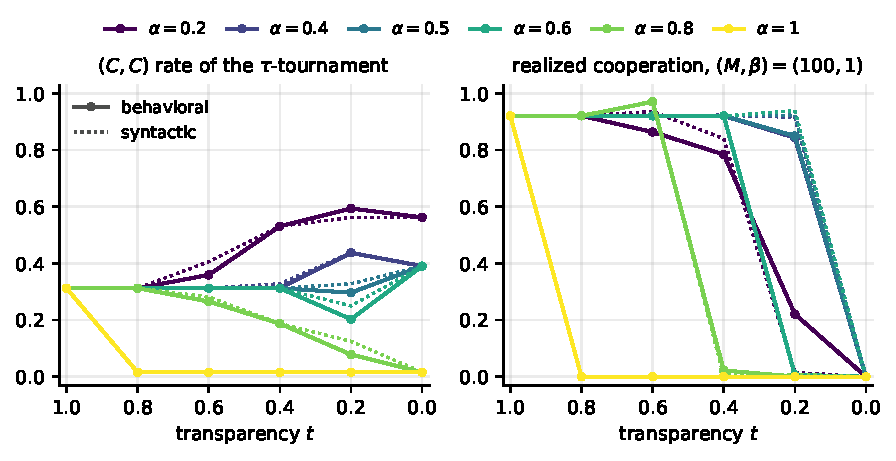
\includegraphics[width=\textwidth]{figures and tables/fig_tau_summary_body}
  \caption{Mutual and realized cooperation rate of the behavioral (solid lines) and syntactic (dotted lines) family, over transparency, one curve per caution $\alpha$, on the \texttt{body} zoo. Left: fraction of ordered pairs that are $(C,C)$. Right: realized cooperation rate of the stationary population at $(M,\beta)=(100,1)$, i.e.\ the share of the long run spent as a monoculture whose self-play is $(C,C)$.}
  \label{fig:tau-summary-body}
\end{figure}

% figures and tables/tau_fullcoop_body.tex — fully cooperative Nash component of the tau tournament, body8, behavioral family, PA-S', hinge cells at the engine side (the floor value).
% GENERATED by latex/scripts/gen_tau_body.py — do not edit by hand.
% Requires: booktabs, xcolor with colortbl (\cellcolor).
\begin{table}[t]\centering\small
\caption{Existence of a fully cooperative Nash component in the $\tau$-tournament on the eight-bot zoo, behavioral family, hinge cells at the engine side (the floor value): the number of connected components of extreme Nash equilibria that contain an equilibrium with cooperation rate exactly $1$ (never more than one). Where it exists, its equilibria are mixtures of \texttt{CooperateBot}, \texttt{DupocBot} and \texttt{TitForTatBot}; a superscript names the programs that join that support at the point. Each row is one caution $\alpha$, each column one transparency $t$; the $t = 1$ column is the base matrix.}
\label{table:tau-ne-fullcoop-body}
\begin{tabular}{@{}lcccccc@{}}\toprule
$\alpha \backslash t$ & $1$ & $0.8$ & $0.6$ & $0.4$ & $0.2$ & $0$ \\\midrule
0.20 & \cellcolor{green!30}1 & \cellcolor{green!30}1 & \cellcolor{green!30}1 & \cellcolor{green!30}1$^{+\mathrm{Cup}}$ & 0 & 0 \\
0.40 & \cellcolor{green!30}1 & \cellcolor{green!30}1 & \cellcolor{green!30}1 & \cellcolor{green!30}1 & \cellcolor{green!30}1 & 0 \\
0.50 & \cellcolor{green!30}1 & \cellcolor{green!30}1 & \cellcolor{green!30}1 & \cellcolor{green!30}1 & \cellcolor{green!30}1 & 0 \\
0.60 & \cellcolor{green!30}1 & \cellcolor{green!30}1 & \cellcolor{green!30}1 & \cellcolor{green!30}1 & 0 & 0 \\
0.80 & \cellcolor{green!30}1 & \cellcolor{green!30}1 & \cellcolor{green!30}1 & 0 & 0 & 0 \\
1.00 & \cellcolor{green!30}1 & 0 & 0 & 0 & 0 & 0 \\\bottomrule
\end{tabular}
\end{table}


% figures and tables/tau_phase_body.tex — stochastically stable set at (M, β) = (100, 1), body8, both channels, PA-S', hinge cells at the engine side (the floor value).
% GENERATED by latex/scripts/gen_tau_body.py — do not edit by hand.
% Requires: booktabs, xcolor with colortbl (\cellcolor).
\begin{table}[t]\centering\small
\caption{Stochastically stable set at $(M,\beta)=(100,1)$ on the eight-bot zoo, hinge cells at the engine side (the floor value), behavioral family; where the syntactic family selects a different set the cell is shaded and reads \enquote{behavioral / syntactic}. \enquote{---} means no type reaches the stability threshold.}
\label{table:tau-phase-body}
\begin{tabular}{@{}lcccccc@{}}\toprule
$\alpha$ & $t = 1$ & $0.8$ & $0.6$ & $0.4$ & $0.2$ & $0$ \\\midrule
0.20 & \textbf{Dup} & \textbf{Dup} & \textbf{Dup} & \cellcolor{orange!25}Def+\textbf{Dup}\,/\,\textbf{Dup} & Def & Def+OB \\
0.40 & \textbf{Dup} & \textbf{Dup} & \textbf{Dup} & \textbf{Dup} & \textbf{Dup} & Def+\textbf{Dup}+OB \\
0.50 & \textbf{Dup} & \textbf{Dup} & \textbf{Dup} & \textbf{Dup} & \textbf{Dup} & Def+\textbf{Dup}+OB \\
0.60 & \textbf{Dup} & \textbf{Dup} & \textbf{Dup} & \textbf{Dup} & \cellcolor{orange!25}\textbf{Dup}+OB\,/\,\textbf{Dup} & Def+\textbf{Dup}+OB \\
0.80 & \textbf{Dup} & \textbf{Dup} & \cellcolor{orange!25}\textbf{Dup}+TFT\,/\,\textbf{Dup} & \cellcolor{orange!25}\textbf{Dup}\,/\,\textbf{Dup}+OB & \cellcolor{orange!25}\textbf{Dup}\,/\,\textbf{Dup}+OB & --- \\
1.00 & \textbf{Dup} & --- & --- & --- & --- & --- \\\bottomrule
\end{tabular}
\end{table}


\begin{figure}[t]
  \centering
  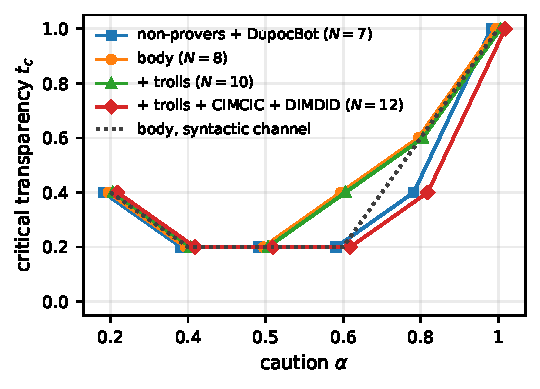
\includegraphics[width=0.75\textwidth]{figures and tables/fig_tau_ladder}
  \caption{Critical transparency $t_c(\alpha)$ on the four nested zoos, behavioral family, hinge cells at the floor side: the lowest transparency on the grid $t \in \{0, 0.2, \dots, 1\}$ at which the realized cooperation of the evolved population at $(M,\beta)=(100,1)$ is still at least $\tfrac12$. Dotted: \texttt{body} under the syntactic channel, which leaves the behavioral threshold at $\alpha = 0.6$ only.}
  \label{fig:tau-ladder}
\end{figure}


\begin{figure}[t]
  \centering
  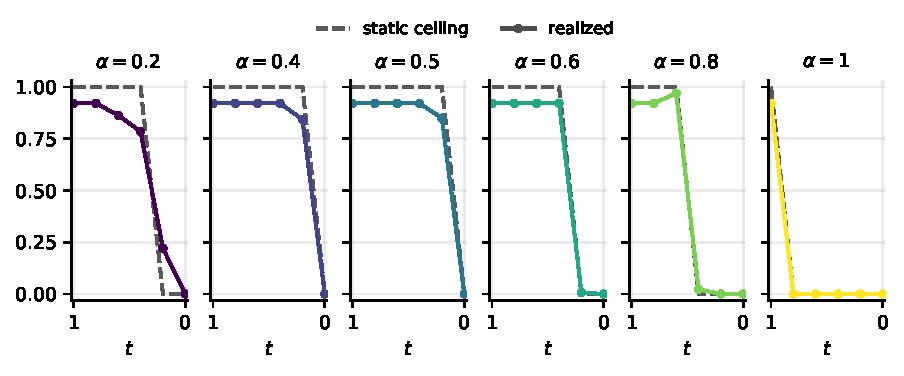
\includegraphics[width=\textwidth]{figures and tables/fig_tau_collapse_body}
  \caption{Static versus dynamic collapse, \texttt{body} zoo, behavioral family, one panel per caution $\alpha$. Dashed: the static ceiling, 1 if a fully cooperative Nash equilibrium exists at that $t$ and 0 otherwise. Solid: the cooperation rate actually reached by the evolved population at $(M,\beta)=(100,1)$. The two lines drop at the same $t$ in every panel.}
  \label{fig:tau-collapse-body}
\end{figure}

\paragraph{The ladder under transparency.}
Is the threshold a property of the zoo? \Cref{fig:tau-ladder} repeats the behavioral sweep on the four nested zoos of \cref{tab:zoo-ladder} and reports $t_c(\alpha)$ for each. For critical transparency $t_c(\alpha)$, \texttt{body} plus the two trolls agrees with \texttt{body}: trolls change nothing, because a troll that defects against one literal program is, under any blur, a defector the Löbian test already handles. For higher caution, the seven-bot zoo and the top rung does move the threshold towards less transparency, but only by a fifth. For the largest zoo for example, with \texttt{CIMCIC} in the roster, the Löbian niche is held by two programs, which share the stochastically stable set wherever the population cooperates, and a cautious population makes do with one grid step less transparency. So part of the signal mass a blurred \texttt{DupocBot} loses to its neighbors now lands on a program that still certifies cooperation. This thus shows that zoo dependency is very low, showing robustness of our results with regards to this axis.

\subsubsection{Summary}
On the eight-bot \texttt{body} zoo, Löbian cooperation thus needs about a fifth of the information about the opponent's identity, measured as normalized mutual information, provided the population is neither too trusting nor too cautious; the threshold rises on both sides of that window. Above the transparency threshold \texttt{DupocBot} is what a population converges to, exactly as at full transparency, and it cooperates at 0.92 against a static ceiling of 1; below it, cooperation stops being an equilibrium and stops being selected at the same transparency, under either channel. The threshold is only scarcely affected by the roster. The selection result of \cref{section:Results-Base} therefore survives the loss of most of the information about the opponent. Critch's framework is stated at full transparency because that is where the proofs are; the population-level conclusion only needs a small amount of it.

\section{Conclusion}
\label{Conclusion}

% Acknowledgements and Disclosure of Funding should go at the end, before appendices and references

\acks{All acknowledgements go at the end of the paper before appendices and references.
Moreover, you are required to declare funding (financial activities supporting the
submitted work) and competing interests (related financial activities outside the submitted work).
More information about this disclosure can be found on the JMLR website.} \boldred{See and do}


\bibliography{sample}

\appendix
\crefalias{section}{appendix}












\section{Proofs}\label{sec:app:proof}

This Appendix collects all proofs from the main paper, divided by section.

\subsection{Proof of Section~\ref{sec:theory}}

\begin{proof}[Proof of Theorem~\ref{th:NE-is-PE}]
Let $\bm{a}^* \in A \times A$ be a NE of $G$. Fix a player $i$ and a deviation $\pi_i\in\Sigma$. Since the opponent's constant program always outputs $a_{-i}^*$, let $b_i:=\operatorname{run}(\pi_i\parallel a_{-i}^*)\in A$. Then
\[
U_i(\pi_i,a_{-i}^*)
= u_i(b_i,a_{-i}^*)
\le u_i(a_i^*,a_{-i}^*)
= U_i(a_i^*,a_{-i}^*),
\]
where the inequality follows because $\bm{a}^*$ is a Nash equilibrium of $G$. Thus no unilateral program deviation is profitable, and $\bm{a}^*$ is a Program equilibrium.
\end{proof}

\begin{proof}[Proof of Theorem~\ref{th:NE-is-tau-PE}]
Since constant programs ignore their input, $\operatorname{run}(a \| \mu) = a$ for all $a \in A$ and $\mu \in \Delta(\Sigma)$. In particular, $\operatorname{outcome}^\tau(\bm{a}^*) = \bm{a}^*$, and hence $U_i^\tau(\bm{a}^*) = u_i(\bm{a}^*)$ for each $i \in I$. Fix $i \in I$ and a deviation $\pi_i' \in \Sigma$, and set $b \coloneqq \operatorname{run}\bigl(\pi_i' \mathrel{\|} \tau_i(a_{-i}^*)\bigr) \in A$. The opponent's constant program outputs $a_{-i}^*$ whatever belief $\tau_{-i}(\pi_i')$ it receives, so
\begin{equation*}
  U_i^\tau(\pi_i', a_{-i}^*) = u_i(b, a_{-i}^*).
\end{equation*}

($\Leftarrow$) If $\bm{a}^*$ is a Nash equilibrium of $G$, then $u_i(b, a_{-i}^*) \le u_i(\bm{a}^*) = U_i^\tau(\bm{a}^*)$, so $\pi_i'$ is not a profitable deviation. Since $i$ and $\pi_i'$ were arbitrary, $\bm{a}^*$ is a $\tau$-Program Equilibrium.

($\Rightarrow$) For every $b \in A$, the constant program $b$ belongs to $\Sigma$ and satisfies $U_i^\tau(b, a_{-i}^*) = u_i(b, a_{-i}^*)$. If $\bm{a}^*$ is a $\tau$-Program Equilibrium, then $u_i(b, a_{-i}^*) \le U_i^\tau(\bm{a}^*) = u_i(\bm{a}^*)$ for all $i \in I$ and $b \in A$, that is, $\bm{a}^*$ is a Nash equilibrium of $G$.
\end{proof}

\begin{proof}[Proof of Theorem~\ref{th:mimic}]
    Let $\bm{\pi}$ be a pure $\tau$-PE with outcome $\bm{a}$. Define $\mu \coloneq \tau_i(\pi_{-i})$ and let $x \in \mathrm{BR}_i(a_{-i})$. Let $\rho$ satisfy Definition~\ref{def:mimic} for $(\pi_i, \mu, x)$. Then by $2.$
    \begin{equation*}
        \mathrm{run}(\rho \| \mu) = x,
    \end{equation*}
    and by $1.$
    \begin{equation*}
         \mathrm{run}(\pi_{-i} \| \tau_{-i}(\rho)) = \mathrm{run}(\pi_{-i} \| \tau_{-i}(\pi_{i})) = a_{-i}.
    \end{equation*}
    The equilibrium condition then implies that
    \begin{equation*}
        u_i(a_i, a_{-i}) = U_i^\tau(\bm{\pi}) \ge U_i^\tau(\rho, \pi_{-i}) = u_i(x, a_{-i}) = \mathrm{max}_{a' \in A}u_i(a', a_{-i}).
    \end{equation*}
    Finally, if both players can mimic, applying this argument to $i = 1$ and $i = 2$ shows that $\bm{a}$ is a pure Nash equilibrium of $G$. Conversely, by Theorem~\ref{th:NE-is-tau-PE}, every pure Nash equilibrium of $G$ is the outcome of a pure $\tau$-PE, namely the profile of the corresponding constant programs.
\end{proof}


\newpage


\section{Theory}
\label{apx-section:Theory}

\subsection{Efficiency assumptions of S}
\label{apx-subsection:Theory-EffAssOfS}
\begin{definition}[Efficiency assumptions]\label[definition]{def:apx-efficiency}
Following \citet[Appendix~B]{Critch}, $S$ satisfies:
\begin{enumerate}
\item[(a)] $S$ can write down expressions that represent arbitrary computable functions; in particular, for every program $\pi$ there is a formula expressing \enquote{$\pi$ run on input $x$ outputs $a$}, which is what a hypothesis such as \enquote{\texttt{opp(DupocBot(k)) == C}} abbreviates;
\item[(b)] $S$ can write down the number $k$ using $\mathcal{O}(\lg k)$ characters;
\item[(c)] $S$ allows abbreviations to be defined and expanded in the middle of proofs;
\item[(d)] there is a constant $e^{*}$, the \emph{proof expansion constant}, such that for every proof $\rho$ of length $k$ there is a proof of length at most $e^{*} \cdot k$ that checks every step of $\rho$ and thereby establishes that $\rho$ is a valid proof.
\end{enumerate}
\end{definition}
Assumption (d) is what turns a proof into evidence \emph{inside} $S$: if $\rho$ proves $\varphi$ in $k$ characters, then $S$ proves $\Box_k \varphi$ in about $e^{*} k$ characters. \citet{Critch_pblt} allows any increasing computable expansion function $e(k)$; since proofs in real proof systems can be checked in linear time, \citet{Critch} take $e(k) = e^{*} k$, and so do we. Assumption (b) is what makes the growth condition $f(k) \succ \mathcal{O}(\lg k)$ of \cref{thm:pblt} the right one: writing the budget down must not by itself consume the budget.

\subsection{Proof of Transposition of statements about programs}
\label{apx-subsection:Theory-ProofTransposePrograms}
\begin{definition}[Names of programs]\label{def:names}
Programs are coded by numbers (\cref{subsection:Lean-FormalSystem}), and $\hat\tau$ acts on codes by exchanging the two action values. For a program $A$, let $\mathrm{rep}(A)$ be the smaller of the codes of $A$ and $\hat\tau A$, the \emph{representative} of the pair $\{A, \hat\tau A\}$; note that $\mathrm{rep}(\hat\tau A) = \mathrm{rep}(A)$. The \emph{name} of $A$ is the closed term
\[
  \overline{A} \;:=\; \mathrm{reval}\big(u_A,\, w_A,\, \dot{\mathrm{rep}}(A)\big),
\]
where $\dot{\mathrm{rep}}(A)$ is a term denoting $\mathrm{rep}(A)$ built from the arithmetical symbols alone, $\mathrm{reval}(u, w, x)$ is the arithmetical function that replaces, in the code $x$, every action value $0$ by $u$ and every action value $1$ by $w$, and the pair $(u_A, w_A)$ is $(c_C, c_D)$ if $A$ is its own representative, $(c_D, c_C)$ if $\hat\tau A$ is, and the numerals $(0, 1)$ if $A = \hat\tau A$. Under the standard reading, $\overline{A}$ denotes the code of $A$ in all three cases. The sentence $\ulcorner A(B) = a\urcorner$ is $\mathrm{Eval}(\overline{A}, \overline{B}, c_a)$, where $\mathrm{Eval}$ is the arithmetical formula expressing \enquote{the first program, run on the second, outputs the third}.
\end{definition}

\begin{proof}[Proof of \cref{prop:bridge}]
The formula $\mathrm{Eval}$ and the term $\dot{\mathrm{rep}}(A)$ are written in the arithmetical symbols only, so $\tau$ leaves them unchanged; it acts on the sentence $\mathrm{Eval}(\overline{A}, \overline{B}, c_a)$ by exchanging $c_C$ and $c_D$ in $u_A, w_A, u_B, w_B$ and in $c_a$. Now $\tau c_a = c_{\tau a}$, and since $\mathrm{rep}(\hat\tau A) = \mathrm{rep}(A)$, the pair $(\tau u_A, \tau w_A)$ is exactly $(u_{\hat\tau A}, w_{\hat\tau A})$: if $A$ is its own representative then $\hat\tau A$ is not, and $(c_C, c_D)$ becomes $(c_D, c_C)$; symmetrically in the other case; and in the case $A = \hat\tau A$ the pair consists of numerals, which $\tau$ fixes. Hence $\tau\overline{A} = \overline{\hat\tau A}$, likewise for $B$, and $\tau\,\mathrm{Eval}(\overline{A}, \overline{B}, c_a) = \mathrm{Eval}(\overline{\hat\tau A}, \overline{\hat\tau B}, c_{\tau a})$.
\end{proof}




\subsection{Additional results and refutations of \citet{Critch}}
\label{apx-subsection:Theory-AddResultsCritch}

\subsubsection{Unexploitability}
\label{apx-subsubsection:Theory-AddResultsCritch-Unexploitability}

We call a program $\pi$ \emph{unexploitable} if no opponent $\pi'$ can get $\mathrm{outcome}(\pi, \pi') = (C, D)$, i.e. whenever $\pi$ cooperates, its opponent cooperates back. The only property of $S$ we need is soundness: if \texttt{proof\_search} finds a proof of a hypothesis, then the hypothesis is true.

The idea is simple. A program that cooperates \emph{only after proving that its opponent cooperates with it} can never be exploited: the proof it found guarantees the opponent's cooperation. We state this once and then check which programs have that shape.

\begin{lemma}\label{lem:apx-guard-witness}
Suppose that every path on which $\pi$ cooperates goes through a successful call \texttt{proof\_search(k, opp, $\varphi$)}, and that the truth of $\varphi$ guarantees that \texttt{opp} cooperates against $\pi$. Then $\pi$ is unexploitable.
\end{lemma}
\begin{proof}
If $\pi$ cooperates against $\pi'$, the search succeeded, so $S$ proved $\varphi$ about $\pi'$. By soundness $\varphi$ is true, so by assumption, $\pi'$ cooperates against $\pi$. The outcome is $(C,C)$.
\end{proof}

\begin{proposition}
\texttt{DefectBot}, \texttt{DupocBot} and \texttt{CIMCIC} are unexploitable.
\end{proposition}
\begin{proof}
\texttt{DefectBot} never cooperates, so there is nothing to show. 

For \texttt{DupocBot(k)}: $\varphi$ = \enquote{\texttt{opp} cooperates against \texttt{DupocBot(k)}}. This is exactly what the lemma asks for.

For \texttt{CIMCIC(k)}: $\varphi$ = \enquote{if \texttt{CIMCIC(k)} cooperates, then \texttt{opp} cooperates against it}. We are in the case where \texttt{CIMCIC(k)} does cooperate, so the \enquote{if} part holds, and the \enquote{then} part follows.
\end{proof}

Note that although \texttt{OBot} looks unexploitable in \cref{table:outcome-matrix-body}, it is not in general (take \texttt{OBotTrollBot} for example). Unexploitability is a property of self-referential guards, which is one more reason the Löbian programs are the ones that survive in \cref{section:Results-Base}.


\subsubsection{DIMCID}
\label{apx-subsubsection:Theory-AddResultsCritch-DIMCID}

\citet{Critch} introduces, next to \texttt{CIMCIC}, the bot \texttt{DIMCID}: \enquote{defect if my cooperation implies your defection} \citep[\S5.2]{Critch}. In $S'$ we prove that \texttt{DIMCID} defects against \emph{every} closed program (\cref{thm:Theory-DIMCID-Defects}), so that it is behaviorally equivalent to \texttt{DefectBot}. This directly contradicts Example 5.3(a) of \citet{Critch}, which gives $\mathrm{outcome}(\texttt{DIMCID}(k), \texttt{CB}) = (C,C)$ where we obtain $(D,C)$; the argument used there for Theorem 5.5(a) on the self-play cell would also yield $(D,C)$ instead of $(C,C)$, which supports our reading.

\begin{theorem}[\texttt{DIMCID} always defects]\label{thm:Theory-DIMCID-Defects}
For every program $\pi$ there is a $k_0$ such that for all $k > k_0$,
\[
  \mathrm{outcome}\bigl(\texttt{DIMCID}(k), \pi\bigr) = (D, \cdot),
\]
and the guard of \texttt{DIMCID}$(k)$ is provable in $S'$ within length $k$.
\end{theorem}

\begin{proof}
Write $p$ for \enquote{\texttt{DIMCID}$(k)$ defects against $\pi$} and $q$ for \enquote{$\pi$ defects against \texttt{DIMCID}$(k)$}. The bot searches for a proof of $\neg p \to q$, which is $p \vee q$, and defects exactly when it finds one, so its action is the fixed point of
\[
  p \;\leftrightarrow\; \Box_k (p \vee q).
\]
Since $p \to p \vee q$, we have $\Box_k p \to \Box_k(p \vee q)$, and the fixed point turns the right-hand side into $p$; hence $\Box_k p \to p$. Löb's theorem (\cref{thm:pblt}) then gives $p$, for large $k$, whatever $q$ is. In words, a proof of the guard makes the bot defect, which falsifies the antecedent $\neg p$, which makes the guard true, and the opponent never enters.
\end{proof}


\subsubsection{Other open problems of \citet{Critch}}
\label{apx-subsubsection:Theory-AddResultsCritch-OpenProblems}
Three further open problems of \citet{Critch} are addressed by the library. We state for each what is proved and what remains.

\paragraph{Open Problem 5: $\mathrm{outcome}(\texttt{CUPOD}(k), \texttt{CIMCIC}(k))$.}
\citet{Critch} rules out $(D,C)$, since \texttt{CupodBot} never exploits, and leaves $(C,C)$, $(C,D)$ and $(D,D)$ open. In $S'$ the cell is a genuine floor with two nested hinges (\cref{subsection:Lean-Floors}): $G_k$, \enquote{\texttt{CIMCIC}$(k)$ proves within length $k$ that its cooperating implies \texttt{CupodBot}$(k)$'s}, and $U_k$, \enquote{\texttt{CupodBot}$(k)$ proves within length $k$ that \texttt{CIMCIC}$(k)$ defects}. We prove, for all large $k$, that $G_k$ gives $(C,C)$, that $\neg G_k \wedge U_k$ gives $(D,D)$, and that $\neg G_k \wedge \neg U_k$ gives $(C,D)$. These are exactly Critch's three cases, so the open problem is not closed but reduced: each hinge is a bounded-consistency question, and the floor side of our matrix, which takes both hinges negative, reports $(C,D)$, both searches failing.
\cref{table:dupoc-row}

\paragraph{Open Problem 6: $\mathrm{outcome}(\texttt{DUPOC}(k), \texttt{DIMCID}(k))$.}
Settled, with no hinge: $(D,D)$ for all large $k$. By \cref{thm:Theory-DIMCID-Defects}, \texttt{DIMCID}$(k)$ always defects; \texttt{DupocBot}$(k)$'s guard, \enquote{\texttt{DIMCID}$(k)$ cooperates with me}, is then false in $\mathbb{N}$, so by soundness no proof of it exists at any length and \texttt{DupocBot}$(k)$ defects.

\paragraph{Open Problem 9.} A computationally bounded \texttt{PrudentBot}: \enquote{Cooperates iff I prove within length $k$ both that my opponent cooperates with me and that my opponent defects against \texttt{DefectBot}.} It exists, and its row is in the library (\cref{tab:prudent-row}).

\input{figures and tables/prudentbot_row}

\subsection{Partial Transparency}
\subsubsection{Signals}
\label{apx-subsubsection:Theory-PartialTrans-Signals}
Fix a finite zoo $\mathcal{Z} = \{\pi_1, \ldots, \pi_n\}$ of admissible programs and assume that $\mathrm{outcome}(\pi_i,\pi_j)$ is known for every ordered pair. A signal $s$ is a function $s\colon \mathcal{Z} \to \Delta(\mathcal{Z})$ that maps a program to a distribution of programs over the zoo.

In \cref{section:Results-Transparency}, we use two families of signals, which we formally define now:

\begin{definition}[Softmax-based signal family]\label{def:App-Softmax-Family}
Consider a pseudo-distance $d : \mathcal{Z} \times \mathcal{Z} \to \mathbb{R}_{\ge 0}$. Then for a temperature $T > 0$, we consider the softmax-based signal family $s_d^T$ to be defined as the Gibbs distribution (softmax) over $Z$:
\[
  \big(s^{T}_{d}(\pi_j)\big)_\ell
  := \frac{\exp\bigl(-d(\pi_j,\pi_\ell)/T\bigr)}
          {\sum_{m=1}^{n} \exp\bigl(-d(\pi_j,\pi_m)/T\bigr)},
  \qquad \pi_\ell \in \mathcal{Z},
\]

As is usual with the Gibs distribution, we set $s^{\infty}_{d}(\pi_j) = \mathrm{unif}_{\mathcal{Z}}$ and $s^{0}_{d}(\pi_j) = \delta_{\pi_j}$.

In our experiments, we take the following two specific pseudo-distances: \begin{itemize}
    \item \textbf{Hamming distance on rows.} For $\mathrm{row}(\pi_j) := (\pi_j(\pi_1),\dots,\pi_j(\pi_n))$,
    \[
    d_{\mathrm{beh}}(\pi_j,\pi_\ell) := \bigl|\{\pi_m \in \mathcal{Z} : \pi_j(\pi_m) \neq \pi_\ell(\pi_m)\}\bigr| \in \{0,\dots,n\}
    \] which is only a pseudo-distance because two different programs can have equal rows. We call the resulting family the \textbf{behavioral family}.
    \item \textbf{Normalized Zhang-Shasha tree edit distance on ASTs.} Let $\mathrm{ast}(\pi)$ be the abstract syntax tree (AST) of $\pi$'s source (the \texttt{Prog}/\texttt{Formula} constructors as node labels, budget arguments erased),
    $|{\cdot}|$ its node count, and $\mathrm{ted}$ the Zhang--Shasha tree edit distance with unit insert, delete and relabel costs \citep{tree_signal_family}. Then we define the normalized Zhang-Shasha tree edit distance on ASTs,
    \[
    d_{\mathrm{syn}}(\pi_j,\pi_\ell) := \frac{\mathrm{ted}\bigl(\mathrm{ast}(\pi_j),\mathrm{ast}(\pi_\ell)\bigr)}
                                           {\max\bigl(|\mathrm{ast}(\pi_j)|,|\mathrm{ast}(\pi_\ell)|\bigr)} \in [0,1]
    \] which is only a pseudo-distance because the ASTs are budget blind (e.g. $\mathrm{ast}(Bot(k)) = \mathrm{ast}(Bot(k'))$, $\forall k, k'$). We call the resulting family the \textbf{syntactic family}.
\end{itemize}
\end{definition}


\begin{definition}[$\varepsilon$-uniform family]\label{def:App-Epsilon}
For $\varepsilon \in [0,1]$, we define the $\epsilon$-uniform family $s^\epsilon(\cdot)$ to be the linear interpolation between the point-mass distribution $\delta_\cdot$ and the uniform distribution over the zoo $\mathrm{unif}_{\mathcal{Z}}(\cdot)$,
\[
  s^{\varepsilon}(\pi_j) = (1-\varepsilon)\,\delta_{\pi_j} + \varepsilon\,\mathrm{unif}_{\mathcal{Z}}(\pi_j).
\]

Unlike the distance-based families it is identity-based: every program is confused with every other at the same rate, the channel matrix is symmetric, and there are no twins, so its
transparency reaches $1$ on every zoo.
\end{definition}

\subsubsection{Measuring Transparency}
\label{apx-subsubsection:Theory-PartialTransparency-Dials}
With signals defined, we move on to defining the tranparency metric we use throughout the experiments.

\begin{definition}[Transparency and calibration]\label{def:App-Calibration}
For a channel $s : \mathcal{Z} \to \Delta(\mathcal{Z})$, its \emph{transparency} is the normalized
mutual information between the true opponent $B \sim \mathrm{unif}_{\mathcal{Z}}$ and the signal
$S \sim s(B)$,
\[
  t(s) := \frac{I(B;S)}{\log_2 n}
        = \frac{1}{n\log_2 n}\sum_{j,\ell} s(\pi_j)(\pi_\ell)\,
          \log_2\frac{s(\pi_j)(\pi_\ell)}{\frac{1}{n}\sum_{k} s(\pi_k)(\pi_\ell)} \in [0,1].
\]
For each family, we set either $T$ or $\varepsilon$ accordingly (using bisection) to obtain a specific transparency $t$. At matched $t$ all three families carry the same amount of information about the opponent and differ only in their confusion structure.
\end{definition}

\section{Lean}
\textit{Not in order at the moment:}
\subsection{Lean implementation}
\label{apx-subsubsection:Lean-Implementation-Encoding}
\paragraph{Programs as numbers.} \textcolor{red}{[Add this somewhere]} The programs above are syntax trees, but the system they reason in is arithmetic, which speaks only about numbers. Each program is therefore identified with a natural number, its \emph{code}: a constructor is a tag paired with the codes of its arguments, for instance
\[
  \ulcorner \texttt{.search}\ k\ \varphi\ p\ q \urcorner \;=\; \langle 6, \langle k, \langle \ulcorner\varphi\urcorner, \langle \ulcorner p\urcorner, \ulcorner q\urcorner\rangle\rangle\rangle\rangle + 1,
  \qquad\text{where}\quad \langle x, y\rangle := (x+y)^2 + y .
\]
The pairing is injective and the tags are distinct, so a code determines its program, and a sub-program always has a smaller code than its parent. We choose this pairing for one reason: it is written with $+$ and $\times$ alone, so it is a term of the language of arithmetic. The code of a program is then the value of a \emph{term} built from the numerals of its leaves, and a program of budget $k$ can be named inside a sentence by a short expression in which $k$ appears as a binary numeral, of length $O(\log k)$. This is assumption~(b) of \citet{Critch}, and \cref{subsection:Lean-FormalSystem} shows that it is not a convenience: a searcher whose own name is longer than its budget can never find a proof about itself.


\subsection{Cupod vs Dupoc}
\label{apx-subsection:Lean-Dupoc}
correspondence table: each pen-and-paper lemma of §3.2 $\iff$ the Lean declaration name and file, plus the verbatim statements (not proofs) of the top-level theorem and the two or three key lemmas (Pf.transpose, the equivariance proposition, outcomeDupocBotvsCupodBot).

\subsection{Taubots}
\label{apx-subsection:Lean-Taubots}

\section{Experiments}
This final appendix regroups all additional details and experiments done in the paper.
\subsection{Metrics}
\label{apx-subsection:Experiments-EGTMetrics}
In \cref{section:Results-Base} and \cref{section:Results-Transparency}, we use three evolutionary stages. Here, we define them prosaically and specify which parameters were used for the experiments. All of them take as input the payoff matrix $A_{PD}$ of \cref{subsubsection:Results-Base-Analysis}, built from the certified outcome cells, and none of them is specific to open-source game theory: they are standard tools of evolutionary game theory. They answer three successive questions: what rational play allows, where a population ends up, and which strategies it keeps returning to.
\begin{itemize}
    \item \textbf{Extreme Nash equilibria} \citep{nash1950equilibrium,nash1951}. The first (and most studied optimum in game theory) we use is Nash Equilibria: which mixtures of zoo strategies are equilibria, and what actions do they play. The mixed Nash equilibria of a bimatrix game form a finite union of polytopes, determined by their vertices, the \emph{extreme} equilibria. We enumerate them in exact rational arithmetic following \citet{enumerateNE}, using Gambit \citep{gambit}, group them into connected components, and record for each component the highest probability of mutual cooperation it supports. This is the ceiling on cooperation that rationality permits, against which the dynamic results are read.
    \item \textbf{Moran process} \citep{Moran_1958,Nowak}. An equilibrium says nothing about whether a population of programs reaches it. The \emph{Moran process} asks that question. It keeps a population of $M$ individuals, each playing one program of the zoo, and at every step does three things: it picks one individual to reproduce, with probability proportional to its fitness $e^{\beta u}$, where $u$ is the individual's average payoff against the current population and $\beta$ sets how strongly payoff matters; it picks one individual uniformly at random to die; and it replaces the latter by a copy of the former. Because the choices are random, a better-earning program can still go extinct by bad luck, and a program that is gone never returns: on its own, the step always ends in a monoculture. Mutation is a separate, rare event that restarts it: a single individual of another program, chosen uniformly among the other $N-1$, appears in the monoculture and the step then decides whether it takes over or dies out. We take the small-mutation limit, in which this is settled before the next mutant appears \citep{Nowak}, so the population is a monoculture almost all of the time and moves from the monoculture of $i$ to that of $j$ with probability $\rho(j \to i)/(N-1)$, where $\rho(j \to i)$ is the probability that one mutant $j$ takes over a population of $i$. The long-run result is a stationary distribution over the programs: the fraction of time the population spends as a monoculture of each one, whatever the start. We compute it for $M \in \{10, 50, 100\}$ and $\beta \in \{0.01, 0.1, 1\}$; the main text reports $(M,\beta) = (100,1)$, strong selection in a population large enough for selection to dominate drift.

    \item \textbf{Stochastic stability} \citep{stochasticEGD,evolutionOfConventions}. The stationary distribution from above gives every strategy some mass. We then look at which strategies are robust: a strategy is stochastically stable if it keeps positive mass as the noise vanishes, that is, if the population keeps returning to it in the long run. We use a finite-$\beta$ proxy: a type is called stochastically stable at $(M,\beta)$ when its stationary mass is at least $1.5/N$ for $N$ types, one and a half times the share it would have under no selection at all, and we always report the raw distribution so that another cut can be applied. This is the selection answer the main text is after: which strategy a population actually ends up playing.
\end{itemize}


\subsection{Hinge results at full transparency}
\label{apx-subsection:Experiments-BaseBots-Hinge}

% figures and tables/outcome_matrix_full.tex — GENERATED by latex/scripts/gen_outcome_matrix_body.py full from
% app/generated/sprime_outcome_theorems.json (source_digest 14009122582737125074). Do not edit by hand.
% Requires: booktabs, graphicx (rotatebox), xcolor with colortbl (\cellcolor).
\begin{table}[t]\centering\scriptsize
\colorlet{ccfill}{green!18}\colorlet{ddfill}{black!12}\colorlet{hlfill}{yellow!35}\colorlet{hgfill}{orange!40}
\providecommand{\cc}{\cellcolor{ccfill}CC}\providecommand{\dd}{\cellcolor{ddfill}DD}
\providecommand{\cd}{CD}\providecommand{\dc}{DC}\providecommand{\hg}[1]{\cellcolor{hgfill}#1$^{\ddagger}$}
\setlength{\tabcolsep}{3pt}
\begin{tabular}{@{}lcccccccccccc@{}}\toprule
 & \rotatebox{90}{\texttt{CooperateBot}} & \rotatebox{90}{\colorbox{hlfill}{\texttt{DefectBot}}} & \rotatebox{90}{\texttt{TitForTatBot}} & \rotatebox{90}{\texttt{DBot}} & \rotatebox{90}{\colorbox{hlfill}{\texttt{OBot}}} & \rotatebox{90}{\texttt{EBot}} & \rotatebox{90}{\colorbox{hlfill}{\texttt{DupocBot}}} & \rotatebox{90}{\texttt{CupodBot}} & \rotatebox{90}{\texttt{CupodTrollBot}} & \rotatebox{90}{\texttt{DupocTrollBot}} & \rotatebox{90}{\colorbox{hlfill}{\texttt{CIMCIC}}} & \rotatebox{90}{\texttt{DIMDID}} \\\midrule
\texttt{CooperateBot} & \cc & \cd & \cc & \cd & \cc & \cd & \cc & \cc & \cc & \cc & \cc & \cc \\
\colorbox{hlfill}{\texttt{DefectBot}} & \dc & \dd & \dd & \dc & \dd & \dd & \dd & \dd & \dc & \dc & \dd & \dd \\
\texttt{TitForTatBot} & \cc & \dd & \cc & \dc & \cd & \dc & \cc & \cc & \cc & \cc & \cc & \cc \\
\texttt{DBot} & \dc & \cd & \cd & \dd & \cd & \cd & \hg{CD} & \cc & \dc & \dc & \hg{CD} & \cc \\
\colorbox{hlfill}{\texttt{OBot}} & \cc & \dd & \dc & \dc & \dd & \dc & \dd & \hg{DC} & \cc & \cc & \dd & \dd \\
\texttt{EBot} & \dc & \dd & \cd & \dc & \cd & \cc & \hg{CD} & \cc & \dc & \dc & \hg{CD} & \cc \\
\colorbox{hlfill}{\texttt{DupocBot}} & \cc & \dd & \cc & \hg{DC} & \dd & \hg{DC} & \cc & \dc & \hg{DC} & \dd & \cc & \hg{DC} \\
\texttt{CupodBot} & \cc & \dd & \cc & \cc & \hg{CD} & \cc & \cd & \dd & \dd & \cc & \hg{CD} & \dd \\
\texttt{CupodTrollBot} & \cc & \cd & \cc & \cd & \cc & \cd & \hg{CD} & \dd & \cc & \cc & \hg{CD} & \cc \\
\texttt{DupocTrollBot} & \cc & \cd & \cc & \cd & \cc & \cd & \dd & \cc & \cc & \cc & \hg{CD} & \cc \\
\colorbox{hlfill}{\texttt{CIMCIC}} & \cc & \dd & \cc & \hg{DC} & \dd & \hg{DC} & \cc & \hg{DC} & \hg{DC} & \hg{DC} & \cc & \hg{DC} \\
\texttt{DIMDID} & \cc & \dd & \cc & \cc & \dd & \cc & \hg{CD} & \dd & \cc & \cc & \hg{CD} & \dd \\\bottomrule
\end{tabular}
\caption{Outcome matrix of the twelve bots of the ladder zoos of \cref{tab:zoo-ladder} in $S'$ — the eight-bot \texttt{body}, the two trolls and the two implication provers — at a shared proof budget $k$ (every searcher on the row and the column receives the same $k$); a cell gives the row bot's action first. Cells hold for every sufficiently large $k$ and every sufficient fuel; each white, green or grey cell is a theorem of $S'$ (\cref{chapter:lean}). Shaded cells: mutual cooperation (green) and mutual defection (grey). Orange cells$^{\ddagger}$ rest on the hinge of \cref{section:Results-Base}: $S'$ proves a dichotomy, and the value shown is the engine side (the floor guard not provable within budget); the other branch gives \texttt{CIMCIC}--\texttt{CupodBot} DC $\to$ CC; \texttt{CIMCIC}--\texttt{CupodTrollBot} DC $\to$ CC; \texttt{CIMCIC}--\texttt{DBot} DC $\to$ CC; \texttt{CIMCIC}--\texttt{DIMDID} DC $\to$ DD; \texttt{CIMCIC}--\texttt{DupocTrollBot} DC $\to$ CC; \texttt{CIMCIC}--\texttt{EBot} DC $\to$ CC; \texttt{CupodBot}--\texttt{OBot} CD $\to$ DD; \texttt{CupodTrollBot}--\texttt{DupocBot} CD $\to$ CC; \texttt{DBot}--\texttt{DupocBot} CD $\to$ CC; \texttt{DIMDID}--\texttt{DupocBot} CD $\to$ DD; \texttt{DupocBot}--\texttt{EBot} DC $\to$ CC. Highlighted names (yellow) are the bots never exploited within this zoo on the engine side, i.e.\ those whose row contains no CD cell: \texttt{DefectBot}, \texttt{OBot}, \texttt{DupocBot}, \texttt{CIMCIC}; on the hinge side the set is \texttt{DefectBot}, \texttt{OBot}, \texttt{DupocBot}, \texttt{CIMCIC}, \texttt{DIMDID}.}
\label{table:outcome-matrix-full}
\end{table}


In \cref{section:Results-Base}, we introduce which programs we analyze (outcomes grouped in \cref{table:outcome-matrix-full}). However, recall that some outcomes depend on a hinge (\cref{subsection:Lean-Floors}), and every number of \cref{section:Results-Base} takes the three hinge pairs at the floor side. On the matrix itself the hinge moves six of the 64 cells, mostly toward cooperation: 24 cells are $(C,C)$ instead of 20 and 18 are $(D,D)$ instead of 16, with 35 row actions $C$ instead of 34. We re-ran the same stages with them at the hinge side; \cref{tab:hinge-body} puts the two branches side by side. The qualitative answer does not move: the three Nash components are still present (with two additional ones), and at strong selection \texttt{DupocBot} is still the only stochastically stable strategy, at every $M$. What moves is the margin. \texttt{DupocBot} no longer exploits \texttt{DBot} and \texttt{EBot}, so its row loses two units of the temptation payoff; \texttt{TitForTatBot}, which already cooperated with both, closes part of the gap and ties it at two of the nine points. The stationary share at $(100, 1)$ falls from 86\% to 71\%, and the self-cooperating share of the long run drops from 0.92 to 0.84. Thus Löbian cooperation is slightly less dominant, but the dynamics stay the same.
% figures and tables/hinge_body_compare.tex — the eight-bot zoo (body8) at t = 1 under both branches of its three hinge dichotomies.
% Sources: app/generated/egt/runs/body8_sprime_t100_a030_ddbeab7343c4 (floor side) and body8_sprime_hinge_side_t100_a030_125c88740d9d (hinge side);
% EGT_FINDINGS_SPRIME.md §8.4. "self-cooperating share" = stationary mass of the types whose self-play cell is (C,C).
\begin{table}[t]
\centering
\begin{tabular}{lcc}
\toprule
\texttt{body}, $t = 1$ & floor side & hinge side \\
\midrule
Nash components (extreme equilibria) & 3 (21) & 5 (16) \\
\texttt{DupocBot} share at $(M,\beta) = (100, 1)$ & 85.9\% & 71.2\% \\
\texttt{DefectBot} share at $(100, 1)$ & 4.5\% & 8.3\% \\
$(M,\beta)$ points where \{\texttt{DupocBot}\} is the selected set & 8 / 9 & 5 / 9 \\
self-cooperating share of the long run at $(100, 1)$ & 0.92 & 0.84 \\
\bottomrule
\end{tabular}
\caption{The eight-bot zoo at full transparency under the two branches of its three hinge dichotomies. Floor side: the floor guards are not provable within budget (the engine's stipulation, the value of \cref{table:outcome-matrix-body}). Hinge side: they are. On the hinge side \texttt{TitForTatBot} ties \texttt{DupocBot} at $(50, 0.1)$ and $(100, 0.01)$, and no type is stochastically stable at the two weakest points.}
\label{tab:hinge-body}
\end{table}



\subsection{Partial Transparency}
The experiments of \cref{section:Results-Transparency} on partial transparency depend on multiple factors that we ablate here.

\subsubsection{The syntactic channel}
\label{apx-subsubsection:Experiments-Transparency-Channels}
An important axis of partial transparency is what signal is blurred. The main paper's experiments focus on behavioral blurring, using the Hamming distance (\cref{def:App-Softmax-Family}) but we argue here that confounding syntax instead (using AST-based tree-editing) leads to the same experimental results. The figures and tables of \cref{section:Results-Transparency} already carry that second channel through the dotted curves of \cref{fig:tau-summary-body} and \cref{fig:tau-ladder}, and the orange cells of \cref{table:tau-ne-fullcoop-body} and \cref{table:tau-phase-body}. By construction this signal carries exactly as much information as the behavioral family at the same $t$ (\cref{def:App-Calibration}); it differs only in \emph{which} programs it mixes up, and one important pair it confuses that the behavioral family does not is \texttt{DupocBot} and \texttt{CupodBot}, one swapped action leaf with opposite dispositions.


On \texttt{body} the difference is minor and only confined to the transparency collapse band at $t=0.6$. Above it the two channels give the same tournament rates to within a few hundredths, the same stochastically stable set, and the same cooperating population; every disagreement sits at or below $t = 0.6$, where the signal is already degraded. The critical transparency $t_c$ is the same under both channels at every caution but one: at $\alpha = 0.6$, where syntactic blur keeps both the cooperative equilibrium and a cooperating population one grid step longer than behavior blur does. The cooperative component is also the same for all but two cells $(\alpha,t)=(0.6, 0.2)$ and $(\alpha,t)=(0.2, 0.4)$. Wherever the two channels differ above the collapse, syntactic blur is the \emph{more} forgiving one: the population cooperates at a higher rate under it at every such point, and the single point where behavior blur does better lies below the collapse under both. So the mechanism by which syntactic blur could be the harsher channel is present on this zoo, and its weight is not enough to make it so anywhere on the grid. Thus different channels produce near-identical results, making them robust to different modes of transparency.



\subsubsection{Aggregators under blur}
\label{apx-subsubsection:Experiments-Transparency-Aggregators}
Another design choice that can influence the results is the aggregator design. How should a Löbian program \emph{vote} once identities blur? In our experiments, we use the $\mathrm{sum}$ operator. Here, we investigate two other aggregators: $\mathrm{min}$ and $\mathrm{max}$. More precisely, the zoo \texttt{body+natives} adds to \texttt{body} two programs that ask \texttt{DupocBot}'s question of every hypothesis, \enquote{does this hypothesis provably cooperate with me?}, and change only the vote: \texttt{MaxConfidenceBot} cooperates iff \emph{at least one} hypothesis of weight at least $\alpha$ passes the test, \texttt{MinConfidenceBot} iff \emph{every} hypothesis of weight at least $1-\alpha$ passes it, so that a single credible hypothesis that cannot be shown to cooperate vetoes. Both are behavioral and syntactic twins of \texttt{DupocBot}, so the comparison runs on the $\varepsilon$-uniform family, which has no twin ceiling. 

On \texttt{body+natives} under the $\varepsilon$-uniform family (\cref{table:tau-aggregators}), the Löbian class \{\texttt{DupocBot}, \texttt{Max}, \texttt{Min}\} holds nearly all of the long run in an even split as long as the signal is clear: the aggregator is irrelevant until blur reaches the thresholds. Below that the three separate in a fixed order. \texttt{MinConfidenceBot}, which any credible hypothesis it cannot certify vetoes, exits first; then, in a mid-blur band, \texttt{MaxConfidenceBot} alone holds the population, because the sum player is fooled into cooperating with blurred exploiters while the max player, which needs one hypothesis credible on its own, is not. \texttt{MaxConfidenceBot} is thus the most robust of all the three, pulling through at very low transparency. At moderate transparency level however, all three aggregators are equal. 


% figures and tables/tau_aggregators.tex — the three aggregators over DupocBot's test on body8 + natives, PA-S', engine side, epsilon family.
% GENERATED by latex/scripts/gen_tau_ladder.py — do not edit by hand.
\begin{table}[t]\centering\small
\caption{Stationary shares at $(M,\beta)=(100,1)$ on the eight-bot zoo plus the two native aggregators, $\varepsilon$-uniform family, hinge cells at the engine side. The three aggregators over \texttt{DupocBot}'s test: \enquote{sum} is the lift \texttt{DupocBot} itself, \enquote{max} is \texttt{MaxConfidenceBot}, \enquote{min} is \texttt{MinConfidenceBot}; \enquote{Löbian} is their combined share. As hypotheses the three are twins, so at $t = 1$ they are payoff-identical and the share splits evenly; they separate only once the signal blurs. Consecutive transparencies with the same shares and the same stable set are merged into one row. The last column is the stochastically stable set.}
\label{table:tau-aggregators}
\begin{tabular}{@{}llrrrrl@{}}\toprule
$\alpha$ & $t$ & sum & max & min & Löbian & stable set \\\midrule
0.20 & $\ge 0.6$ & 31\% & 31\% & 31\% & 94\% & Dup+Max+Min \\
0.20 & $0.4$ & 42\% & 42\% & 1\% & 85\% & Dup+Max \\
0.20 & $0.2$ & 1\% & 69\% & 1\% & 70\% & Def+Max \\
0.20 & $0$ & 0\% & 33\% & 0\% & 33\% & Def+Max+OB \\\midrule
0.40 & $\ge 0.4$ & 31\% & 31\% & 31\% & 94\% & Dup+Max+Min \\
0.40 & $0.2$ & 42\% & 42\% & 1\% & 85\% & Dup+Max \\
0.40 & $0$ & 0\% & 33\% & 0\% & 33\% & Def+Max+OB \\\midrule
0.50 & $\ge 0.4$ & 31\% & 31\% & 31\% & 94\% & Dup+Max+Min \\
0.50 & $0.2$ & 2\% & 85\% & 0\% & 87\% & Max \\
0.50 & $0$ & 0\% & 33\% & 0\% & 33\% & Def+Max+OB \\\midrule
0.60 & $\ge 0.4$ & 31\% & 31\% & 31\% & 94\% & Dup+Max+Min \\
0.60 & $0.2$ & 1\% & 90\% & 1\% & 92\% & Max \\
0.60 & $0$ & 25\% & 25\% & 0\% & 50\% & Def+Dup+Max+OB \\\midrule
0.80 & $\ge 0.6$ & 31\% & 31\% & 31\% & 94\% & Dup+Max+Min \\
0.80 & $0.4$ & 1\% & 90\% & 1\% & 92\% & Max \\
0.80 & $0.2$ & 44\% & 44\% & 1\% & 89\% & Dup+Max \\
0.80 & $0$ & 17\% & 17\% & 0\% & 33\% & Def+Dup+EB+Max+OB+TFT \\\bottomrule
\end{tabular}
\end{table}


\subsubsection{Hinge results under partial transparency}
\label{apx-subsubsection:Experiments-Transparency-Hinge}
Finally, as for the base case (\cref{apx-subsection:Experiments-BaseBots-Hinge}), we analyze the impact of the hinge in the partial transparency case. We re-ran the two body sweeps of \cref{section:Results-Transparency} with the three hinge pairs at the hinge side. This side is the more cooperative one at every transparency above the collapse: its $(C,C)$ rate starts at 0.38 instead of 0.31 at $t = 1$ and stays above the floor side's by roughly that margin, with the three regimes of \cref{section:Results-Transparency}, rising at low caution, flat in the middle, falling at high caution, unchanged (\cref{fig:tau-summary-body-hinge-side}, left). Below full transparency, the picture is less robust than on the floor side, because of one specific reason: on the hinge side \texttt{CupodBot}'s and \texttt{DupocBot}'s own-action rows coincide, so the behavioral family cannot tell them apart and spreads \texttt{DupocBot}'s mass over the two from the first step below $t = 1$. Under that family the signal a lifted \texttt{DupocBot} receives, when it meets either twin, puts exactly half its mass on a hypothesis it cooperates with, since it defects on \texttt{CupodBot}; the hinge side therefore turns on whether half the mass meets the threshold. For $\alpha \le 0.5$ it does: \texttt{DupocBot} now cooperates with its twin, the two become mutual cooperators and share the stochastically stable set (\cref{table:tau-phase-body-hinge-side}), and the population cooperates as much as on the floor side. For $\alpha \ge 0.6$ it does not: \texttt{DupocBot} defects against \emph{itself}, since it cannot rule out that its opponent is the twin it defects on, Löbian self-cooperation is lost from the first step below full transparency, and realized cooperation collapses (\cref{fig:tau-summary-body-hinge-side}, right).

In short, the hinge changes the picture under partial transparency for one reason only. On the hinge side, \texttt{CupodBot} and \texttt{DupocBot} play the same row of actions, so a signal based on behavior cannot tell them apart, and \texttt{DupocBot} is never sure whether it is facing itself or its twin. Everything that differs from the floor side comes from this: cautious populations lose cooperation early, and the syntactic signal, which still tells the two apart, does not show the effect. The main result is the same on both sides: Löbian cooperation is what selection keeps, and it survives a large loss of information about the opponent. What the hinge changes is only how much information is needed, and that depends on whether the zoo contains such a pair.




\begin{figure}[t]
  \centering
  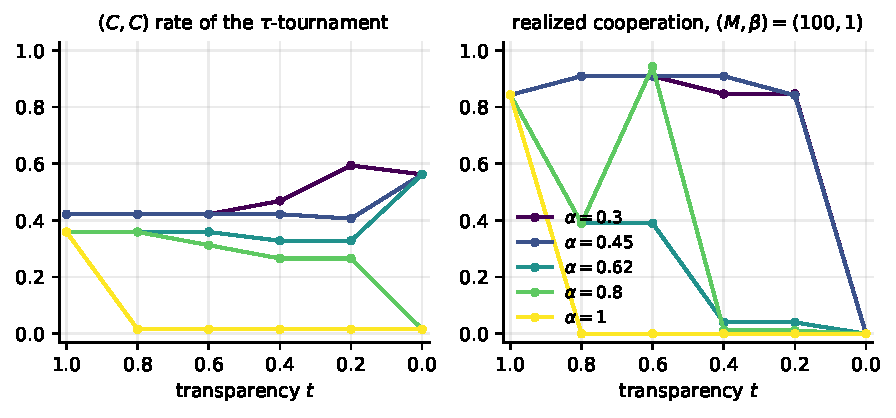
\includegraphics[width=\textwidth]{figures and tables/fig_tau_summary_body_hinge_side}
\caption{Mutual and realized cooperation rate on the eight-bot \texttt{body} zoo with the hinge pairs at the hinge side (solid) and, for comparison, at the floor side (dotted, the values of \cref{fig:tau-summary-body}), behavioral family, one curve per caution $\alpha$: $(C,C)$ rate of the tournament (left) and realized cooperation of the evolved population at $(M,\beta)=(100,1)$ (right).}
  \label{fig:tau-summary-body-hinge-side}
\end{figure}

% figures and tables/tau_phase_body_hinge_side.tex — stochastically stable set at (M, β) = (100, 1), body8, both channels, PA-S', hinge cells at the hinge side.
% GENERATED by latex/scripts/gen_tau_body.py — do not edit by hand.
% Requires: booktabs, xcolor with colortbl (\cellcolor).
\begin{table}[t]\centering\small
\caption{Stochastically stable set at $(M,\beta)=(100,1)$ on the eight-bot zoo, hinge cells at the hinge side, behavioral family; where the syntactic family selects a different set the cell is shaded and reads \enquote{behavioral / syntactic}. \enquote{---} means no type reaches the stability threshold.}
\label{table:tau-phase-body-hinge-side}
\begin{tabular}{@{}lcccccc@{}}\toprule
$\alpha$ & $t = 1$ & $0.8$ & $0.6$ & $0.4$ & $0.2$ & $0$ \\\midrule
0.20 & \textbf{Dup} & \cellcolor{orange!25}Cup+\textbf{Dup}\,/\,\textbf{Dup} & \cellcolor{orange!25}Cup+\textbf{Dup}\,/\,Def+OB & \cellcolor{orange!25}Cup+\textbf{Dup}\,/\,Def & Def & Def+OB \\
0.40 & \textbf{Dup} & \cellcolor{orange!25}Cup+\textbf{Dup}\,/\,\textbf{Dup} & \cellcolor{orange!25}Cup+\textbf{Dup}\,/\,\textbf{Dup} & \cellcolor{orange!25}Cup+\textbf{Dup}\,/\,\textbf{Dup} & \cellcolor{orange!25}Cup+\textbf{Dup}\,/\,Def+OB & Def+OB \\
0.50 & \textbf{Dup} & \cellcolor{orange!25}Cup+\textbf{Dup}\,/\,\textbf{Dup} & \cellcolor{orange!25}Cup+\textbf{Dup}\,/\,\textbf{Dup} & \cellcolor{orange!25}Cup+\textbf{Dup}\,/\,\textbf{Dup} & \cellcolor{orange!25}Cup+\textbf{Dup}\,/\,\textbf{Dup} & Def+OB \\
0.60 & \textbf{Dup} & \cellcolor{orange!25}Def+OB\,/\,\textbf{Dup} & \cellcolor{orange!25}Def+OB\,/\,\textbf{Dup} & \cellcolor{orange!25}OB\,/\,\textbf{Dup} & \cellcolor{orange!25}OB\,/\,\textbf{Dup}+OB & Def+OB \\
0.80 & \textbf{Dup} & \cellcolor{orange!25}Def+OB\,/\,\textbf{Dup} & \cellcolor{orange!25}TFT\,/\,\textbf{Dup} & \cellcolor{orange!25}Def+OB\,/\,OB & \cellcolor{orange!25}Def+OB\,/\,\textbf{Dup}+OB & --- \\
1.00 & \textbf{Dup} & --- & --- & --- & --- & --- \\\bottomrule
\end{tabular}
\end{table}


\end{document}
